% todo General:	
%	Improve Images & Captions
%	Normen, A_k vs A, L2() H1 etc i,j,k index
%   all indicies 
%   L^2 over R/C?!?! H1 H2 the same...
%   Einleitungstexte hinzufügen, wohin und wie
%   Verweis auf Kuchement! Referenzen, andere Cites
%   Semi-Periodic conditions to check! where + or minus
%   compact embedding
%   integral dx everywhere removed? or u(x)
% check all semi perodic conditions
%  Very Important:
% 	http://www.lti.kit.edu/rd_download/EPhys5Fcompl.pdf
%  Important: 
% 	https://nano.tu-dresden.de/~rgutierrez/2008SS_WPV_NM/SolutionKronigPenneyModel1.pdf	
% 	The likelihood that the particle will pass through the barrier is given by the transmission coefficient, whereas the likelihood that it is reflected is given by the reflection coefficient. Schrödinger's wave-equation allows these coefficients to be calculated.
%  Interesting:
% 	http://www.ece.uc.edu/~mcahay/QuantumSystems/KroenigPenney.pdf
% 	http://ecee.colorado.edu/~bart/book/book/chapter2/pdf/ch2_3_8.pdf
\RequirePackage[l2tabu, orthodox]{nag}
\documentclass[11pt]{mitthesis}

\usepackage[utf8]{inputenc}
\usepackage[english]{babel}

\usepackage[export]{adjustbox}
\usepackage[dvipsnames]{xcolor}
\usepackage[colorlinks=false, pdfborder={0 0 0}]{hyperref}

\usepackage{amsmath}
\usepackage{amssymb}
\usepackage{amsthm}
\usepackage{booktabs}
\usepackage{cmap}
\usepackage{csquotes}
\usepackage{dsfont}
\usepackage{enumitem}
\usepackage{lgrind}
\usepackage{mathtools}
\usepackage{mathrsfs}
\usepackage{microtype}
\usepackage{nicefrac}
\usepackage{pgf}
\usepackage{pgfplots}
\usepackage{tikz}
\usepackage{xpatch}

\pgfplotsset{compat=1.7}
\usetikzlibrary{arrows}

\pagestyle{plain}

\makeatletter
  \xpatchcmd{\proof}{\@addpunct{.}}{\@addpunct{:}}{}{}
  \DeclareUnicodeCharacter{00A0}{ } 
  \def\supp{\operatorname{supp}}
  \setlength{\parindent}{0pt}
  \xpatchcmd{\proof}{\@addpunct{.}}{\@addpunct{:}}{}{} 
  \@ifundefined{thechapter}{}{\def\thefigure{\thechapter.\arabic{figure}}} 
\makeatother

\newcommand{\C}{\mathbb{C}}
\newcommand{\K}{\mathbb{K}}
\newcommand{\R}{\mathbb{R}}
\newcommand{\Q}{\mathbb{Q}}
\newcommand{\Z}{\mathbb{Z}}
\newcommand{\N}{\mathbb{N}}


\newtheoremstyle{itshape}{}{}{\itshape}{}{\bfseries}{:}{ }{}
\newtheoremstyle{normal}{}{}{\normalfont}{}{\bfseries}{:}{ }{}
\theoremstyle{itshape}
\newtheorem{theorem}{Theorem}[chapter]
\newtheorem*{remark}{Remark}
%\theoremstyle{normal}
\newtheorem*{definition}{Definition}
\newtheorem*{definitions}{Definitions}
\numberwithin{equation}{chapter}

% temporarily removed all proofs
%\usepackage{environ}
%\NewEnviron{killcontents}{}
%\let\proof\killcontents
%\let\endproof\endkillcontents

\begin{document}

\begin{titlepage}
  
\includegraphics[scale=0.45]{kit-logo.jpg}
  \vspace*{2cm} 

  \begin{center} \large 
    
    Bachelor Thesis
    \vspace*{2cm}

    {\huge On the spectra of the Schrödinger operator with periodic delta potential}
    \vspace*{2.5cm}

    Martin Belica
    \vspace*{0.125cm}

    30 September 2016 % todo Vater Datum
    \vspace*{4.25cm}


    Supervisors: Prof. Dr. Michael Plum,
    \vspace*{0.125cm}
    
    Dr. Andrii Khrabustovskyi \\[1cm]
    Faculty for Mathematics \\[1cm]
	Karlsruhe Institute of Technology
  \end{center}
\end{titlepage}
 
\tableofcontents
\chapter{Introduction} \label{chap1}

The problem considered in this thesis arises from the Kronig-Penney model, see for example \cite[Chap. 3]{HeeringEP}, which describes an idealised quantum-mechanical system that models a quantum particle behaving as a matter wave moving in one-dimension through an infinite periodic array of rectangular potential barriers, i.e. through a space area in which a potential attains a local maximum. Such an array commonly occurs in models of periodic crystal lattices where the potential is caused by ions in the crystal structure. Those charged molecules create an electromagnetic field around themselves. Hence, any particle moving through such a crystal would be subject to a recurrent electromagnetic potential. Although a solid particle, simplified as a point mass, would be reflected at such a barrier, there is a possibility that the quantum particle, as it behaves like a wave, penetrates the barrier and continues its movement beyond. Assuming the spacing between all ions is equidistant the potential function $V(x)$ in the lattice can be approximated by a rectangular potential like this:

\begin{figure}[!ht] \centering
	\resizebox{.55\linewidth}{!}{
		\definecolor{wqwqwq}{rgb}{0.3764705882352941,0.3764705882352941,0.3764705882352941}
		\begin{tikzpicture}[line cap=round,line join=round,>=triangle 45,x=1.0cm,y=1.0cm]
			\draw[->,color=wqwqwq] (-5.5,0.) -- (5.5,0.);
			\foreach \x in {-5.,-4.,-3.,-2.,-1.,1.,2.,3.,4.,5.}
				\draw[shift={(\x,0)},color=wqwqwq] (0pt,-2pt);
			\draw[->,color=wqwqwq] (0.,-1.1) -- (0.,4.25);
			\clip(-5.5,-1.1) rectangle (5.5,4.25);
			\draw (-0.3,3.)-- (0.3,3.);
			\draw (0.3,0.)-- (0.3,3.);
\draw (-0.3,3.)-- (-0.3,0.);
\draw (-1.7,3.)-- (-1.7,0.);
\draw (-2.3,3.)-- (-1.7,3.);
\draw (-2.3,3.)-- (-2.3,0.);
\draw (-1.7,3.)-- (-1.7,0.);
\draw (-3.7,0.)-- (-3.7,3.);
\draw (-3.7,3.)-- (-4.3,3.);
\draw (-4.3,3.)-- (-4.3,0.);
\draw (-3.7,3.)-- (-3.7,0.);
\draw (-3.7,3.)-- (-4.3,3.);
\draw (1.7,3.)-- (1.7,0.);
\draw (1.7,3.)-- (2.3,3.);
\draw (2.3,3.)-- (2.3,0.);
\draw (3.7,0.)-- (3.7,3.);
\draw (3.7,3.)-- (4.3,3.);
\draw (4.3,3.)-- (4.3,0.);
\draw (-3.7,0.)-- (-2.3,0.);
\draw (-1.7,0.)-- (-0.3,0.);
\draw (0.3,0.)-- (1.7,0.);
\draw (2.3,0.)-- (3.7,0.);
\draw (4.3,0.)-- (5.7,0.);
\draw (-4.3,0.)-- (-5.7,0.);
\draw [->] (0.65,1.5) -- (0.65,3.);
\draw [->] (0.65,1.5) -- (0.65,0.);
\draw [->] (0.65,1.5) -- (0.65,3.);
\draw [dotted] (0.3,3.)-- (0.65,3.);
\draw [dotted] (1.,3.)-- (0.65,3.);
\draw [->] (2.75,-0.5) -- (2.3,-0.5);
\draw [->,line width=0.4pt] (1.25,-0.5) -- (1.7,-0.5);
\draw [dotted] (1.7,0.)-- (1.7,-1.);
\draw [dotted] (2.3,0.)-- (2.3,-0.5);
\draw [dotted] (2.3,-0.5)-- (2.3,-1.);
\draw (1.75,-0.041546762589927816) node[anchor=north west] {$b$};
\draw (0.7603430877901116,1.9021582733812952) node[anchor=north west] {$\rho$};
\draw (0.1,4.25) node[anchor=north west,color=wqwqwq] {$V(x)$};
\draw (5,-0.1) node[anchor=north west,color=wqwqwq] {$x$};
\end{tikzpicture}
	}
	\caption{Potential $V(x)$ of the Kronig-Penney model}
\end{figure}

where $b$ is the \enquote{support} and $\rho$ the magnitude of the potential. We are interested in the spectrum of the operator describing the situation of the Kronig-Penney model when the particle moves through periodically distributed, singular potentials. With respect to the above this means taking the limit $b \rightarrow 0$ while $V_{0}$ remains of order $\rho b^{-1}$. 

\section*{Mathematical Basics}

For the upcoming analysis we need some basic concepts from functional analysis and spectral theory are here briefly reviewed:
~\newline ~\newline
Let $C_{0}^{\infty}$ denote the linear space containing all smooth function $f \colon \R \rightarrow \R$ with compact support, i.e. for $f \in C_{0}^{\infty}$ there exists a compact interval $I \subseteq \R$ such that $f(x) = 0$ for all $x \notin I$. And will hereafter $\langle x, x \rangle$ denote the scalar product in $L^{2}(\R)$.
\begin{definition}[Weak derivative]
Let $\Omega \subseteq \R$ be open, and $f \in L^{1}_{loc}(\Omega)$. The function $f$ is said to have the weak derivative $g \in L^{1}_{loc}(\Omega)$ in $\Omega$ if
  \[ - \int_{\Omega} f \varphi' = \int_{\Omega} g \varphi \]
holds for all $\varphi \in C_{0}^{\infty}(\Omega)$.
\end{definition}
Now, an important example for a Hilbert space is the Sobolev space $H^{k}(\Omega)$.
\begin{definition} Let $\alpha \in \N$ and denote with $D^{\alpha} u$ the $\alpha$-th weak derivate of $u$. We call the space
\[ H^{k}(\Omega) \coloneqq \left\{ u \in L^{2}(\Omega) : D^{\alpha} u \in L^{2}(\Omega) \text{ for } 0 \leq \alpha \leq k \right\} \]
equipped with the norm $\| \cdot \|_{H^{k}(\Omega)} \coloneqq \left( \sum_{0 \leq \alpha \leq k} \| D^{\alpha} \cdot \|_{L^{2}(\Omega)}^{2} \right)^{\frac{1}{2}}$ Sobolev space.
\end{definition}
 which is defined to be the set of functions $f$ in $L^{2}(\Omega)$ such that the function $f$ and its weak derivatives up to the order $k$ have a finite $L^{2}(\Omega)$ norm, by admitting the inner product in terms of the $L^{2}(\Omega)$ inner product for all derivatives up to order $k$: 
	\[ \langle u , v \rangle_{H^{k}(\Omega)} = \sum_{i=0}^{k} \left\langle D^{i}u , D^{i} v \right\rangle_{L^{2}(\Omega)}. \] 	

\begin{definition}[Distributions]
	On $C_{0}^{\infty}$ a sequence $(f_{n})$ converges against $f \in C_{0}^{\infty}$ if the support of all members of the sequence is in a compact interval $I \subset \R$, i.e.
	$$ \supp (f_{n}) \subseteq I \quad \forall n \in \N, $$
	and on this interval $f_{n}$ and all its derivatives converge uniformly against $f$, i.e.
	\[ \| f_{n}^{(i)} - f^{(i)} \|_{\infty} \rightarrow 0 \quad \text{ for } n \rightarrow \infty \]
	for all $i \in \N_{0}$. One can proof that this concept of convergence generates a topology on $C_{0}^{\infty}$ and one usually denoted with $\mathcal{D}(\R)$ the space $C_{0}^{\infty}$ equipped with this topology. From now on, we denote with $D'(\R)$ the space of all linear functionals on $C_{0}^{\infty}$ that are continuous with respect to this topology and call those functionals distributions.
\end{definition}

An important example for a distribution is the Dirac delta function $\delta_{x_{0}}$ where $x_{0} \in \R$. It is defined as the limit of a weakly converging sequence of functionals over normed symmetric around $x_{0}$ cumulative distribution functions $\delta_{\epsilon}$, whereas the support of those cumulative distributions converges to zero. It holds $\delta_{x_{0}} = \lim_{\epsilon \rightarrow 0} \delta_{\epsilon}$ in $D'(\R)$. An example for such a sequence is

	\begin{equation}
		\delta_{\epsilon}(x) = \frac{1}{\sqrt{2 \pi} \epsilon} e^{-\frac{x^{2}}{2 \epsilon^{2}}}. \label{smooth-potential}
	\end{equation}
	 
Which implies the definition

	\[ \delta_{x_{0}}(f) \coloneqq \int_{\R} \delta_{x_{0}} f(x) dx \coloneqq \lim_{\epsilon \rightarrow 0} \int_{\R} \delta_{\epsilon}(x - x_{0}) f(x) dx. \]
	
Moreover, is easily seen that $\delta_{x_{0}}(f) = \lim_{\epsilon \rightarrow 0} \delta_{\epsilon}(f) = f(x_{0})$, for a proof see \cite[Chap. 1.4]{WeisST}.

\begin{definitions}
Let $X, Y$ be Banach spaces and let $A \colon \mathcal{D}(A) \rightarrow Y$ be a linear operator with domain $\mathcal{D}(A) \supset X$. 
\begin{enumerate}[label=\alph*\upshape)]
	\item We call $A$ closed if $graph(A) \coloneqq \{ (x, Ax) : x \in \mathcal{D}(A) \} \subseteq X \times Y$ is a closed set.
	\item The operator $A^{*} : \mathcal{D}(A^{*}) \rightarrow H $ is called the adjoint of $A$ and is defined by
		\[ \mathcal{D}(A^{*}) \coloneqq \{ u \in H : \exists u^{*} \in H ~\forall v \in \mathcal{D}(A) \langle u, A v \rangle = \langle u^{*} , v \rangle \} \]
		and $A^{*} u \coloneqq u^{*}$ for $u \in \mathcal{D}(A^{*})$. Note that for $u \in \mathcal{D}(A^{*})$, $u^{*}$ is uniquely determined. 
\end{enumerate}
Are $X, Y$ Hilbert spaces, $\langle \cdot, \cdot \rangle$ denotes the scalar product on $Y$ and $A$ a bounded operator, we call
\begin{enumerate}[label=\alph*\upshape)]  \setcounter{enumi}{1}
	\item $A$ symmetric, if $\langle Tx,y \rangle = \langle x ,Ty \rangle$ for all $x,y \in \mathcal{D}(A)$, and
	\item $A$ self-adjoint, if $A$ is densely defined on $X$ and coincides with its adjoint.
\end{enumerate}
Furthermore, let $I$ denote the identity operator on $X$ and $A$ be a linear, bounded and closed operator.
	\begin{enumerate}[label=\alph*\upshape)] \setcounter{enumi}{3}
		\item $\lambda \in \C$ belongs in the resolvent set of $A$, $\lambda \in \rho(A)$, if
			\[  A  - \lambda I \colon \mathcal{D}(A) \rightarrow X \text{ bijective, i.e. } (A - \lambda I)^{-1} \colon X \rightarrow \mathcal{D}(A) \text{ is a bounded linear operator,} \]
		\item $\sigma(A) = \C \setminus \rho(A)$ is called the spectrum of $A$, and
		\item $\lambda \in \rho(A) \rightarrow R(\lambda, A) = (A - \lambda I)^{-1}$ is the resolvent function of $A$.
	\end{enumerate}		
\end{definitions}

Finally, in chapters \ref{chap3}, \ref{chap5} we will examine so called compact operators and some of their properties.

\begin{definition}
	Let $X$ be a normed space and $Y$ a Banach space. A linear operator $A \colon X \rightarrow Y$ is called compact, if $T(U_{X})$ is relativ compact in $Y$.
\end{definition}

Additionally, throughout this thesis we will need some theorems and lemmata from functional analysis and spectral theory, which will be listed in the appendix.
\chapter{\texorpdfstring{The Schrödinger operator $A$}{The Schrödinger operator A}}

The above introduced problem  can be modelled by a one-dimensional Schrödinger operator where the potential is given by a delta-distribution. Thereby the operator $A$ is formally defined through the operation\pdfcomment{do I have to explain why?}
\begin{equation}
	- \frac{d^{2}}{dx^{2}} + \rho \sum_{i \in \Z} \delta_{x_{i}} \label{the-operator-A-formally}
\end{equation}
on the whole of $\R$, where $\delta_{x_{i}}$ denotes the Dirac delta distribution in $x_{i}$ and $x_{i}$ are periodically distributed points on $\R$. $\Omega_{k}$ will hereafter identify the periodicity cell containing delta point $x_{k}$ and let w.o.l.g. $x_{0} = 0$ and $a \coloneqq |\Omega_{i}| = 1$ for all $i \in \Z$.
~\\ ~\\
In general, one cannot expect that \eqref{the-operator-A-formally} has a classical
solution. For the existence of a classical solution, all the problem has to be sufficiently regular, which for a distributional potential is never the case. Nevertheless, for $\mu \in \R$ the problem
\begin{equation}
	\int u' \overline{v'} + \rho \sum_{i \in \Z} u(x_{i}) \overline{v(x_{i})} - \mu \int u \overline{v} = \int f \overline{v} \quad \forall v \in H^{1}(\R), \label{weak-formulation-of-A}
\end{equation}	
where $u \in H^{1}(\R)$ and $f \in L^{2}$ requires much less regularity, as it is the weak-formulation of our operator $A$ shifted by the constant $\mu$.
~\\ ~\\
We should note that left-hand side of problem \eqref{weak-formulation-of-A} is actually convergent, as for arbitrary $\tilde{x}_{i} \in \Omega_{i}$
\begin{eqnarray}
	\sum_{i \in \Z} |u(x_{i})|^{2} & \leq & \sum_{i \in \Z} \left( \big| u(\tilde{x}_{i}) + \int_{\tilde{x}_{i}}^{x_{i}} u'( \tau ) d\tau \big| \right)^{2} \notag \\
		 & \leq & 2 \sum_{i \in \Z} \left( \int_{\Omega_{i}} |u( x )|^{2} dx +  \int_{\Omega_{i}} \left| u'(\tau) \right|^{2} d\tau \right) \notag \\
		 & \leq & 2 \cdot \| u \|^{2}_{H^{1}(\R)}. \label{estimation-for-potential}
\end{eqnarray}

We will now examine show that for each $f \in L^{2}(\R)$ the equation \eqref{weak-formulation-of-A} has a unique solution. Given $f \in L^{2}(\R)$, we define a functional $l \colon H^{1} \rightarrow \R$ through Riesz' Representation Theorem with
	\[ l(v) \coloneqq \int_{\R} f v \]
and the bilinear form $B_{\mu} \colon H^{1}(\R) \times H^{1}(\R) \rightarrow \R$ for $\mu \in \R$ through
	\[ B_{\mu}[u, v] \coloneqq \int u' \overline{v'} + \rho \sum_{i \in \Z} u(x_{i}) \overline{v(x_{i})} - \mu \int u \overline{v}. \]
Such that \eqref{weak-formulation-of-A} is equivalent to finding $u \in H^{1}(\R)$ such that
	\begin{equation}
		B_{\mu}[u, v] =  l(v) \quad \forall v \in H^{1}(\R). \label{weak-formulation-of-A-for-LM}
	\end{equation}
The existence of an unique $u \in H^{1}(\R)$ satisfying \eqref{weak-formulation-of-A-for-LM} follows from Lax Milgram's Theorem asserts if the bilinear form $B$ is bounded and coercive, which we will prove in the next theorem.

\begin{theorem} \label{2.1:thm-LaxMilgram}
	The bilinear form $B_{\mu}[u, v]$ as left-hand of \eqref{weak-formulation-of-A} has for all $u, v \in H^{1}(\R)$ the properties
	\begin{enumerate}
		\item[i)] $B_{\mu}[u, v]$ is bounded, i.e. there exists a constant $\alpha > 0$ such that
			\[ \left| B_{\mu}[u,v] \right| \leq \alpha \|u\| \|v\| \quad (u, v \in H^{1}(\R)) \]
		\item[ii)] $B_{\mu}[u, u]$ is coercive, i.e. there exists a constant $\beta > 0$ such that
			\[ \beta \|u\|^{2} \leq B_{\mu}[u, u] \quad (u \in H^{1}(\R)). \]
	\end{enumerate} 

	\begin{proof} ~\\
		i) The boundedness follows from
		\begin{align*}
			|B(u, \varphi)|^{2} & \leq \| u' \| \cdot \| v' \| + 2 \rho \sum_{i \in \Z} |u(x_{i})|^{2} |v(x_{i})|^{2} - \mu \| u \| \cdot \| v \| \\
				& \leq \| u' \| \cdot \| v' \| + 8 \rho \cdot \| u \|^{2}_{H^{1}(\R)} \| v \|^{2}_{H^{1}(\R)}  - \mu \| u \| \cdot \| v \| \\
				& = (8\rho - \mu) \| u \| \cdot \| v \| + 8\rho \left( \| u \| \cdot \| v' \| + \| u' \| \cdot \| v \| \right) + (8\rho + 1) \| u' \| \cdot \| v'\| \\
				& \leq \alpha \cdot \| u \|_{H^{1}} \cdot \| \varphi \|_{H^{1}}
		\end{align*}
		ii)
		For the coercivity assume first $\rho \geq 0$, in order that for $\mu < -1$:
		\begin{align*}
			B(u, u) & = \langle u' , u' \rangle + \rho \sum_{i \in \Z} u(x_{i})^{2} - \mu \langle u , u \rangle \\
					& \geq \langle u' , u' \rangle - \mu \langle u , u \rangle \geq \langle u' , u' \rangle  + \langle u , u \rangle \\
					& = \| u \|_{H^{1}}^{2}.
		\intertext{Same for $\rho < 0$, where $\mu < 2\rho$:}
			B(u, u) & = \langle u' , u' \rangle + \rho \sum_{i \in \Z} |u(x_{i})|^{2} - \mu 	\langle u , u \rangle \\
					& = \langle u' , u' \rangle + \rho \sum_{i \in \Z} \big| u(\tilde{x}_{i}) + \int_{\tilde{x}_{i}}^{x_{i}} u(x) dx \big|^{2} - \mu \langle u , u \rangle \\
					& \geq \langle u' , u' \rangle + 2 \rho \left( \int_{\R} |u(x)|^{2} dx + \int_{\R} |u'(\tau)|^{2} d\tau \right) - \mu \langle u , u \rangle \\
					& = (2 \rho + 1) \| u' \|^{2} + (2\rho - \mu) \| u \|^{2}  \\
					& \geq \beta \| u \|_{H^{1}}^{2},
		\end{align*}
	\end{proof}
\end{theorem}
Thus, there is a function $u \in H^{1}(\R)$ as the unique solution to the problem \eqref{weak-formulation-of-A-for-LM} for fixed $f \in L^{2}(\R$ and the operator $R_{\mu} \colon L^{2}(\R) \rightarrow H^{1}(\R), f \mapsto u$ is for $\mu \in \R$ small enough well-defined; obviously this mapping is one-to-one since for $u_{1} = u_{2}$
	\begin{equation}
		0 = B_{\mu}[u_{1}, v] - B_{\mu}[u_{2}, v]= \int (f_{1} - f_{2}) \overline{v} \quad \forall v \in H^{1}(\R). \label{f1f2almosteverywhere}
	\end{equation} 
As further $H^{1}(\R)$ is dense in $L^{2}(\R)$ this yields that the equation \eqref{f1f2almosteverywhere} holds also for all $v \in L^{2}(\R)$ and therefore $f_{1} = f_{2}$ almost everywhere. Accordingly $R_{\mu}$ is bijective and in return we can now define the Schrödinger operator as follows
		\[ A \coloneqq R_{\mu}^{-1} + \mu I \]
from which additionally follows that $R_{\mu}$ is the resolvent of $A$.

\section{\texorpdfstring{The Domain of $A$}{The Domain of A}}
Lax Milgram's Theorem guarantees a solution $u \in H^{1}(\R)$ of \eqref{weak-formulation-of-A}, nevertheless the operator $A$ yields additional properties about such a solution, more specifically about the domain of $A$. For every fixed $k \in \Z$ we therefore consider in \eqref{weak-formulation-of-A} a test function $v \in C^{\infty}(\R)$ such that $\supp v = \Omega_{k}$, then
	\[ \int_{x_{k}-\nicefrac{1}{2}}^{x_{k}} u'(x) \overline{v'(x)} dx = \int_{x_{k}-\nicefrac{1}{2}}^{x_{k}} A u \overline{v} \iff \int_{x_{k}-\nicefrac{1}{2}}^{x_{k}} u(x) \overline{v''(x)} dx = \int_{x_{k}-\nicefrac{1}{2}}^{x_{k}} - A u \overline{v}, \]
such that $A u = - u'' \in L^{2}$ on $(x_{k} -\nicefrac{1}{2}, x_{k})$ and analogous on $(x_{k}, x_{k} + \nicefrac{1}{2})$.
As $k \in \Z$ was arbitrary this means 
	$$ \mathcal{D}(A) \subset \big\{ u \in \bigcap_{i \in \Z} \left( H^{2}(x_{i}-\nicefrac{1}{2}, x_{i}) \cap H^{2}(x_{i}, x_{i} + \nicefrac{1}{2}) \right) \big\}. $$
	
Next, a test function $v \in C^{\infty}(\R)$ sucht that $\supp v = \Omega_{k}$ will yield for an arbitrary $k \in \Z$ from \eqref{weak-formulation-of-A}   through integration by parts on both sides of $x_{k}$ that
	\[ -\left( \int_{x_{k}-\nicefrac{1}{2}}^{x_{k}} + \int_{x_{k}}^{x_{k} + \nicefrac{1}{2}}\right) u'' \cdot \overline{v} + \left( u'(x_{k}-0) \overline{v(x_{k})} - u'(x_{k} + 0) \overline{v(x_{k})} \right) \\ \]
	\[ +  \rho u(x_{k})\overline{v(x_{k})} = - \int_{x_{k} - \nicefrac{1}{2}}^{x_{k}} u'' \overline{v} - \int_{x_{k}}^{x_{k} + \nicefrac{1}{2}} u'' \overline{v}. \]
But as we chose $v \in C^{\infty}(\R)$ this is equivalent to
	\[ u'(x_{k}-0) - u'(x_{k}+0) + \rho u(x_{k}) = 0, \]
such that
	\begin{equation}
		\mathcal{D}(A) \subset \Big\{ u \in \bigcap_{i \in \Z} H^{2}(x_{i}, x_{i + 1}) : u'(x_{i} - 0) - u'(x_{i} + 0) + \rho u(x_{i}) = 0 , ~\forall i \in \Z \Big\} \eqqcolon B \label{firstdomaininclusion}
	\end{equation} 
The operator is hence well-defined by the action
	\[ A u = \begin{cases}
					- u'' & (x_{k} - \frac{1}{2}, x_{k}) \\
					- u'' & (x_{k}, x_{k} + \frac{1}{2}),
			 \end{cases} \quad \forall k \in \Z \]
				
We can further prove the opposite inclusion for \eqref{firstdomaininclusion}. As $\mathcal{R}(R_{\mu}) = \mathcal{D}(A)$, we proceed by proving each $u \in B$ is also in the range of $R_{\mu}$. More specifically, as $\mathcal{D}(R_{\mu}) = L^{2}(\R)$ define $f \coloneqq A u$. To show $u = R_{\mu}(f - \mu u)$ consider\pdfcomment{I guess I have to show that $f - \mu$ u is onto though $\mu$ is fixed..}
	\[ \int_{\R} u' \overline{v'} + \rho \sum_{i \in \Z} u(x_{i}) \overline{v(x_{i})} - \mu \int_{\R} u \overline{v}= \int_{\R}(f-\mu u) \overline{v} \]
	\[ \iff \sum_{i \in \Z} \int_{\Omega_{i}} u' \overline{v'} + \rho u(x_{i}) \overline{v(x_{i})} = - \sum_{i \in \Z} \int_{x_{i} - \nicefrac{1}{2}}^{x_{i}} u'' \overline{v} + \int_{x_{i}}^{x_{i} + \nicefrac{1}{2}} u'' \overline{v}. \]
	For each $k \in \Z$ partial integration with a function $v$ having $\supp v = (x_{k} - \nicefrac{1}{2}, x_{k} + \nicefrac{1}{2})$ yields
	\[ \left( \int_{x_{k} - \nicefrac{1}{2}}^{x_{k}} + \int_{x_{k}}^{x_{k} +\nicefrac{1}{2}} \right) u' \overline{v'} - u'(x_{k}-0) \overline{v(x_{k})}  + u'(x_{k}+0) \overline{v(x_{k})}  = \int_{\Omega_{k}} u' \overline{v'} + \rho u(x_{k}) \overline{v(x_{k})} \]
	\[ \iff u'(x_{k}+0) - u'(x_{k}-0) - \rho u(x_{k}) = 0 \]
	such that we conclude
	\begin{align*}
		\mathcal{D}(A) & = \Big\{ u \in H^{1}(\R): u \in \bigcap_{j \in \Z} H^{2}(x_{j} , x_{j+1}), u'(x_{j} - 0) - u'(x_{j} + 0) + \rho \cdot u(x_{j}) = 0 ~\forall j \Big\}.
	\end{align*}
~\newpage % todo temporarily

\section{The self-adjointness}

In chapter 4, we will further utilise the fact that the operator $A$ is self-adjoint. A self-adjoint operator is always closed, symmetric and has a completely real spectrum which narrows our analysis its spectrum down. 

\begin{theorem} \label{2.2:thm-RmuSymmetric}
	$R_{\mu}$ and $R_{\mu}^{-1}$ are both symmetric operator.
	
	\begin{proof}
		First, focus on $R_{\mu}^{-1} = (A - \mu I)$. As for all $v \in D(A)$:
			\begin{align*}
				\langle R_{\mu}^{-1} u, v \rangle & = \langle (A - \mu I) u, v \rangle \\
					& = \int u'\overline{v'} -  \mu \int u \overline{v} + \rho \sum_{i \in \Z} u(x_{i}) \overline{v(x_{i})} \\
					& = \langle u, (A - \mu I) v \rangle = \langle u,  R_{\mu}^{-1} v \rangle.
			\end{align*}

		$R_{\mu}^{-1}$ is symmetric. Now, as $\mathcal{D}(R_{\mu}) = L^{2}(\R)$ and $\mathcal{R}(R_{\mu}) = \mathcal{D}(R_{\mu}^{-1})$ for each $f, g \in L^{2}(\R)$ it follows
		
		\[  \langle R_{\mu} f, g \rangle =  \langle R_{\mu} f, R_{\mu}^{-1} R_{\mu} g \rangle = \langle f, R_{\mu} g \rangle \]
		
		such that $R_{\mu}$ is also symmetric.
	\end{proof}
\end{theorem}

Now, using both symmetries we can show that $A$ is self-adjoint:

\begin{theorem} \label{2.3:thm-ASelfAdjoint}
	$A$ is a self-adjoint operator.
		
	\begin{proof}
		As we already know that $R_{\mu}$ and $R_{\mu}^{-1}$ are symmetric, showing that $R_{\mu}^{-1}$ is self-adjoint is equivalent to showing that if $v \in \mathcal{D}({R_{\mu}^{-1}}^{*})$ and $v^{*} \in L^{2}(\R)$ are such that
		\[ \langle R_{\mu}^{-1} u, v \rangle = \langle u, v^{*} \rangle, \quad \forall u \in \mathcal{D}(R_{\mu}^{-1}) \tag*{(*)} \]
		then $v \in \mathcal{D}(R_{\mu}^{-1})$ and $R_{\mu}^{-1} v = v^{*}$.
		In $(*)$ we define $u \coloneqq R_{\mu} f$ for $f \in L^{2}$ and use that $R_{\mu}$ is symmetric and defined on the whole of $L^{2}(\R)$:
		\[  \langle f, v \rangle = \langle R_{\mu} f, v^{*} \rangle = \langle f, R_{\mu} v^{*} \rangle, \quad \forall u \in \mathcal{D}(R_{\mu}^{-1}) \]
		
		Which means that $v \in \mathcal{R}(R_{\mu}) = \mathcal{D}(R_{\mu}^{-1})$ and $R_{\mu}^{-1} v = v^{*}$, i.e. $R_{\mu}^{-1}$ is self-adjoint. As the operator $A$ is simply $R_{\mu}^{-1}$ shifted by $\mu \in \R$, $A$ is self-adjoint as well.		
	\end{proof}
\end{theorem}
\chapter{Fundamental domain of periodicity and the Brillouin zone}

Let $\Omega$ be the fundamental domain of periodicity associated with \eqref{the-operator-A-formally}, for simplicity let $\Omega = \Omega_{0}$ and thus $x_{0} = 0$ being the delta-point contained in $\Omega$. As commonly used by literature the reciprocal lattice for $\Omega$ is equal to $[-\pi, \pi]$, the so called one-dimensional Brillouin zone $B$. For fixed $k \in \overline{B}$, consider now the operator $A_{k}$ on $\Omega$ formally defined by the operation
		\[ -\frac{d^{2}}{dx^{2}} + \rho \delta_{x_{0}}. \]
	More precisely, define $A_{k}$ by considering the problem to find for $f \in L^{2}(\Omega)$ a function $u \in H^{1}_{k}$ such that
	\[ \int_{\Omega} u' \overline{v'} + \rho u(x_{0}) \overline{v(x_{0})} - \mu \int_{\Omega} u \overline{v} = \int_{\Omega} f \overline{v} \quad \forall v \in H^{1}_{k}, \]
	where 
	\begin{eqnarray}
		H^{1}_{k} & \coloneqq & \Big\{ \psi \in H^{1}(\Omega): ~ \psi(\frac{1}{2}) = e^{ik} \psi(-\frac{1}{2}) \Big\}. \label{quasi-periodic-condition}	
	\end{eqnarray}

 	Due to the fact that convergence in $H^{1}_{k}$ implies the convergence on the trace of $\Omega$, $H^{1}_{k}$ is a closed subspace of $H^{1}(\R)$ and one can apply the same arguments as above to show that now the operator $R_{\mu, k}$ is well-defined and define again % todo define operator
		\[ A_{k} \coloneqq R_{\mu, k}^{-1} + \mu, \] 
	such that $R_{\mu, k}$ is the resolvent of $A_{k}$.	
		
\begin{theorem} \label{3.1:thm-R_mu,k.isCompact}
	The operator $R_{\mu, k}$ is compact.

	\begin{proof}
	For each bounded sequence $(f_{j})_{j \geq 1} \in L^{2}(\Omega)$ there exist $(u_{j})_{j \geq 1} \in H^{1}_{k}$ such that
		\[ u_{j} = R_{\mu, k} f_{j} \quad \forall j \geq 1 \]
	and each $u_{j}$ for $j \geq 1$ has to satisfy
		\begin{equation}
			\int_{\Omega} u_{j}' \overline{v'} + \rho u_{j}(x_{0}) \overline{v(x_{0})} - \mu \int_{\Omega} u_{j} \overline{v} = \int f_{j} \overline{v} \quad \forall v \in H^{1}_{k}. \label{ujsatisfy}
		\end{equation} 
	Now, choosing in \eqref{ujsatisfy} $v = u_{j}$ yields with \eqref{estimation-for-potential} for $\mu$ small enough
		\[  \| u_{j} \|_{H^{1}(\Omega)} \leq \| f_{j} \|_{L^{2}(\Omega)} \| u_{j} \|_{L^{2}(\Omega)} \leq c \sqrt{vol(\Omega)} \]
	Which shows that $(u_{j})_{j \geq 1}$ is bounded in $H^{1}(\Omega)$. As $H^1(\Omega) \subset C(\Omega)$ it holds
		\begin{equation}
			|f(x) - f(y)| \leq c |x - y|^{\nicefrac{1}{2}} \text{ for some } c > 0. \label{eq:H1estimation}
		\end{equation}  
		From \eqref{eq:H1estimation} follows for $f \in B_{H^{1}} \coloneqq \{ f \in H^{1}_{k}(\Omega) : \| f \| \leq 1 \}$ that 
		\[ |f(x)|^{2} \leq 2 \| f \|^{2}_{L^{2}} + 2 \leq 4 \quad \forall x \in \Omega. \]
		Now, given an $\epsilon > 0$ we partition $\Omega$ into $n_{\epsilon}$ equidistant intervals $I_{k}$, i.e. $\Omega = \bigcup_{j = 1}^{n_{\epsilon}} I_{j}$. As all $f \in B_{H^{1}_{k}}$ are by \eqref{estimation-for-potential} uniformly bounded on $\Omega$, there exist for each subinterval $I_{k}$ a finite number of constants $c_{1}(I_{k}), \dotsc, c_{\nu_{\epsilon}}(I_{k})$ such that 
			$$ \forall f \in B_{H^{1}_{k}} ~\exists j \in \{1, \dotsc, \nu_{\epsilon} \}: \quad |f(\frac{k}{n_{\epsilon}}) - c_{j}(I_{k})| < \frac{1}{n_{\epsilon}} \quad \forall k \in \{ 1 , \dotsc, n_{\epsilon} \}. $$	
		Hence, a simple function $g \in L^{2}(\Omega)$ with function value $c_{k}$ on interval $I_{k}$ would yield
		\begin{align*}
			\| f - g \|^{2}_{L^{2}} & = \sum_{k = 0}^{n-1} \int_{\frac{k}{n}}^{\frac{k+1}{n}} | f(x) - c_{k+1} |^{2} dx \\
				& =  2 \sum_{k = 0}^{n-1} \int_{\frac{k}{n}}^{\frac{k+1}{n}} | f(x) - f(\frac{k}{n}) |^{2} dx +  2 \sum_{k = 0}^{n-1} \int_{\frac{k}{n}}^{\frac{k+1}{n}} | f(\frac{k}{n}) - c_{k+1} |^{2} dx \\
				& \leq 2 \sum_{n = 0}^{n-1} \frac{c}{n^{2}} + 2 \sum_{n=0}^{n-1} \frac{1}{n^{3}} = \frac{2}{n} \left( c + \frac{1}{n} \right) < \epsilon^{2} \text{ for } n \text{ small enough.}
		\end{align*}		 
		This means for all $\epsilon > 0$ there exists a finite set of simple functions $\{ g_{1}, \dotsc, g_{N} \}$ such that for all $f \in B_{H^{1}_{k}}$ there exists a $\nu \in \{1, \dotsc, N\}$ such that $\| f - g_{\nu} \| \leq \epsilon$. Together with the closure of $H^{1}_{k}$ this yields the compact embedding of $H^{1}_{k}$ in $L^{2}(\Omega)$ and thus $R_{\mu, k}$ is compact. % todo #4: This, I haven't showed yet...
	\end{proof}	
\end{theorem}		

\section{The Spectrum of $A_{k}$}		
As from now, consider the periodic eigenvalue problem
	\begin{equation}
		A_{k} \psi = \lambda \psi \text{ on } \Omega \text{ for } \psi \in H^{1}_{k}. \label{eigv-problem}
	\end{equation}

In writing the boundary condition in \eqref{quasi-periodic-condition}, we understand $\psi$ extended to the whole of $\R$. In fact, \eqref{quasi-periodic-condition} forms boundary conditions on $\partial \Omega$, so-called semi-periodic boundary conditions. \\
	
Since $\Omega$ is bounded, and $R_{\mu, k}$, as resolvent of $A_{k}$, is a compact and symmetric operator, $A_{k}$ has a purely discrete spectrum satisfying	
	\[ \lambda_{1}(k) \leq \lambda_{2}(k) \leq \dotsc \leq \lambda_{s}(k) \rightarrow \infty \text{ as } s \rightarrow \infty. \]
and the corresponding eigenfunction can be chosen such that they depend on $k$ in a measurable way\footnote{see [M. Reed and B. Simon. Methods of modern mathematical physics I–IV]} and that they form a $\langle \cdot , \cdot \rangle$-orthonormal and complete system $(\psi_{s}(\cdot, k))_{s \in \N}$ of eigenfunctions for \eqref{quasi-periodic-condition}.

Now, we want to transform the eigenvalue problem \eqref{eigv-problem} such that the boundary condition is independent from $k$. Define therefore
	\[ \varphi_{s}(x, k) \coloneqq e^{-ikx} \psi_{s}(x, k). \]
Then,
	\begin{align*}
		A_{k} \psi_{s}(x, k) & = \frac{d^{2}}{dx^{2}} \psi_{s}(x, k)|_{(x_{0} - \frac{1}{2}, x_{0})} \cdot \mathds{1}_{(x_{0} - \frac{1}{2}, x_{0})} + \frac{d^{2}}{dx^{2}} \psi_{s}(x, k)|_{(x_{0}, x_{0}  + \frac{1}{2})} \cdot \mathds{1}_{(x_{0}, x_{0} + \frac{1}{2})} \\
				& = e^{ikx} \left( \frac{d^{2}}{dx^{2}} + ik \right)^{2} \varphi_{s}(x, k)|_{(x_{0} - \frac{1}{2}, x_{0})} \cdot \mathds{1}_{(x_{0} - \frac{1}{2}, x_{0})} \\
				& ~\qquad + e^{ikx} \left( \frac{d^{2}}{dx^{2}} + ik \right)^{2} \varphi_{s}(x, k)|_{(x_{0}, x_{0}  + \frac{1}{2})} \cdot \mathds{1}_{(x_{0}, x_{0} + \frac{1}{2})}.
	\end{align*}
Defining the operator $\tilde{A_{k}} \colon D(A_{k}) \rightarrow L^{2}(\R)$ through 
	\[ \tilde{A}_{k} \varphi_{s}(x, k) \coloneqq \begin{cases}
 		\left( \frac{d^{2}}{dx^{2}} + ik \right)^{2} \varphi_{s}(x, k)|_{(x_{0} - \frac{1}{2}, x_{0})} & \text{for } x \in (x_{0} - \frac{1}{2}, x_{0}) \\ \left( \frac{d^{2}}{dx^{2}} + ik \right)^{2} \varphi_{s}(x, k)|_{(x_{0}, x_{0}  + \frac{1}{2})} & \text{for } x \in (x_{0}, x_{0} + \frac{1}{2})
 	\end{cases} \] 
and using \eqref{eigv-problem} and \eqref{quasi-periodic-condition}, gives
		\[ \varphi_{s}(x - \frac{1}{2}, k) = e^{-ik(x - \frac{1}{2})} \psi_{s}(x - \frac{1}{2}, k) = e^{-ik(x + \frac{1}{2})} \psi_{s}(x + \frac{1}{2}, k) = \varphi_{s}(x + \frac{1}{2}, k). \]
Which shows that $(\varphi_{s}(\cdot, k))_{s \in \N}$ is an orthonormal and complete system of eigenfunctions of the periodic eigenvalue problem
	\begin{eqnarray}
		\tilde{A}_{k} \varphi = & \lambda
		 \varphi \text{ on } \Omega, \label{mod-eigv-problem} \\
		 \varphi(x - \frac{1}{2}) = & \varphi(x + \frac{1}{2}). \label{periodic-condition}
	\end{eqnarray}
with the same eigenvalue sequence $(\lambda_{s}(s))_{s \in \N}$ as in \eqref{eigv-problem}. We shall see that the spectrum of the operator $A$ can be constructed from the eigenvalue sequences $(\lambda_{s}(s))_{s \in \N}$ by varying $k$ over the Brillouin zone $B$.\\
	
\section{The Floquet transormation}
An important step towards this aim is the Floquet transformation
	\begin{equation}
		(Uf)(x, k) \coloneqq \frac{1}{\sqrt{|B|}} \sum_{n \in \Z} f(x - n) e^{ikn} \quad (x \in \Omega, k \in B). \label{floquet-transformation}
	\end{equation}
		
\begin{theorem} \label{3.2:thm-UIsometricIsomorphism}
	$ U \colon L^{2}(\R) \rightarrow L^{2}(\Omega \times B)$ is an isometric isomorphism, with inverse
		\begin{equation}
			(U^{-1}g)(x - n) = \frac{1}{\sqrt{|B|}} \int_{B} g(x, k) e^{-ikn} dk \quad (x \in \Omega, n \in \Z). \label{3.8}
		\end{equation} 
	If $g(\cdot, k)$ is extended to the whole of $\R$ by the semi-periodicity condition \eqref{quasi-periodic-condition}, we have
		\begin{equation}
			U^{-1} g = \frac{1}{\sqrt{|B|}} \int_{B} g(\cdot, k) dk. \label{3.9}
		\end{equation}
		
	\begin{proof}
		For $f \in L^{2}(\R)$,
		\begin{equation}
			\int_{\R} |f(x)|^{2} dx = \sum_{n \in \Z} \int_{\Omega} |f(x - n)|^{2} dx. \label{functionoverperiodicity}
		\end{equation} 
		Here, we can exchange summation and integration by Beppo Levi's Theorem. Therefore, 
		\[ \sum_{n \in \Z} |f(x - n)|^{2} < \infty \text{ for a.e. } x \in \Omega.\]
		Thus, $(Uf)(x, k)$ is well-defined by \eqref{floquet-transformation} (as a Fourier series with variable $k$) for a.e. $x \in \Omega$, and Parseval's equality gives, for these $x$,
		\[ \int_{B}|(Uf)(x,k)|^{2} dk = \sum_{n \in \Z} |f(x - n)|^{2}. \]
		By \eqref{functionoverperiodicity}, this expression is in $L^{2}(\Omega)$, and
		\[ \| Uf \|_{L^{2}(\Omega \times B)} = \|f\|_{L^{2}(\R)}. \]
		We are left to show that $U$ is onto, and that $U^{-1}$ is given by \eqref{3.8} or \eqref{3.9}. Let $g \in L^{2}(\Omega \times B)$, and define
		\begin{equation}
			f(x - n) \coloneqq \frac{1}{\sqrt{|B|}} \int_{B} g(x, k) e^{-ikn} dk \quad (x \in \Omega, n \in\Z).\label{3.11}
		\end{equation}
		For fixed $x \in \Omega$, Parseval's Theorem gives
		\[ \sum_{n \in \Z} |f(x - n)|^{2} = \int_{B} |g(x, k)|^{2} dk, \]
		whence, by integration over $\Omega$,
		\begin{eqnarray}
			\int_{\Omega \times B} |g(x, k)|^{2} dx dk & = \int_{\Omega} \sum_{n \in \Z} |f(x - n)|^{2} dx \\
				& = \sum_{n \in\Z} \int_{\Omega} |f(x-n)|^{2} dx \\
				& = \int_{\R} |f(x)|^{2} dx,	
		\end{eqnarray}
		i.e. $f \in L^{2}(\R)$. Now \eqref{floquet-transformation} gives, for a.e. $x \in\Omega$,
		\[ f(x - n) = \frac{1}{\sqrt{|B|}} \int_{B} (Uf)(x,k) e^{-ikn} dk \quad (n \in \Z), \]
		whence \eqref{3.11} implies $U f = g$ and \eqref{3.8}. Now \eqref{3.9} follows from \eqref{3.8} using $g(x + n, k) = e^{ikn} g(x, k)$.
	\end{proof}				
\end{theorem}

\section{Completeness of the Bloch waves}

Using the Floquet transformation $U$, we are now able to prove a completeness property of the Bloch waves $\psi_{s}(\cdot, k)$ in $L^{2}(\Omega)$ when we vary $k$ over the Brillouin zone $B$.
	
\begin{theorem} \label{3.3:thm-flConvergence}
		For each $f \in L^{2}(\R)$ and $l \in \N$, define
			\begin{equation}
				f_{l}(x) \coloneqq \frac{1}{\sqrt{|B|}} \sum_{s=1}^{l} \int_{B} \langle (Uf)(\cdot, k), \psi_{s}(\cdot, k) \rangle_{L^{2}(\Omega)} \psi_{s}(x, K) dk \quad (x \in \R). \label{3.15}
			\end{equation}
		Then, $f_{l} \rightarrow f$ in $L^{2}(\R)$ as $l \rightarrow \infty$.

	\begin{proof}
		Sine $Uf \in L^{2}(\Omega \times B)$, we have $(Uf)(\cdot, k) \in L^{2}(\Omega)$ for a.e. $k \in B$ by Fubini's Theorem. Since $(\psi_{s}(\cdot, k))_{s \in \N}$ is orthonormal and complete in $L^{2}(\Omega)$ for each $k \in B$, we obtain
			\[ \lim_{l \rightarrow \infty} \| (Uf)(\cdot, k) - g_{l}(\cdot, k) \|_{L^{2}(\Omega)} = 0 \text{ for a.e. } k \in B\]
		where 
			\begin{equation}
				g_{l}(x, k) \coloneqq \sum_{s=1}^{l} \langle(Uf)(\cdot, k), \psi_{s}(\cdot,k)\rangle_{L^{2}(\Omega)} \psi_{s}(x,k). \label{3.16}
			\end{equation}
		Thus, for $\chi(k) \coloneqq \| (Uf)(\cdot, k) - g_{l}(\cdot, k) \|^{2}_{L^{2}(\Omega)}$, we get
			\[ \chi_{l}(k) \rightarrow 0 \text{ as } l \rightarrow \infty \text{ for a.e. } k \in B, \]
		and moreover, by Bessel's inequality,
			\[ \chi_{l}(k) \leq \| (Uf)(\cdot, k) \|^{2}_{L^{2}(\Omega)} \text{ for all } l \in \N \text{ and a.e. } k \in B \]
		and $\|(Uf)(\cdot, k)\|^{2}_{L^{2}(\Omega)}$ is in $L^{1}(B)$ as a function of $k$ by Theorem \ref{3.2:thm-UIsometricIsomorphism}. Altogether, Lebesgue's Dominated Convergence theorem implies
			\[ \int_{B} \chi_{l}(k) dk \rightarrow 0 \text{ as } l \rightarrow \infty, \]
		i.e., 
			\begin{equation}
				\| U f - g_{l} \|_{L^{2}(\Omega \times B)} \rightarrow 0 \text{ as } l \rightarrow \infty \label{3.17}
			\end{equation} 
		Using \eqref{3.15}, \eqref{3.16} and \eqref{3.9}, we find that $f_{l} = U^{-1}g_{l}$, whence \eqref{3.17} gives
			\[ \| U(f - f_{l}) \|_{L^{2}(\Omega \times B)} \rightarrow 0 \text{ as } l \rightarrow \infty,\]
		and the assertion follows since $U \colon L^{2}(\R) \rightarrow L^{2}(\Omega \times B)$ is isometric by Lemma \ref{3.2:thm-UIsometricIsomorphism}.
	\end{proof}
\end{theorem}
\chapter{The Floquet transformation and the Bloch waves} \label{chap3.5}

In chapter \ref{chap4} we will show that the spectrum of the operator $A$ can be constructed from the eigenvalue sequences $(\lambda_{s}(k))_{s \in \N}$ introduced above by varying $k$ over the Brillouin zone $B$. For this purpose we will need two results involving the Floquet transformation to be able to move the problem from $L^{2}(\R)$ to $L^{2}(\Omega \times B)$ whereas $\Omega \times B$ is compact by assumption. For the sake of completeness, we include here the proofs of both theorems, as given in \cite[Chap. 3.4, 3.5]{Plum10}.

\section{Properties of the Floquet transformation}

\begin{theorem} \label{3.2:thm-UIsometricIsomorphism}
	The Floquet transformation $U \colon L^{2}(\R) \rightarrow L^{2}(\Omega \times B)$ 
	\begin{equation}
		(Uf)(x, k) \coloneqq \frac{1}{\sqrt{|B|}} \sum_{n \in \Z} f(x - n) e^{ikn} \quad (x \in \Omega, k \in B). \label{floquet-transformation}
	\end{equation}
	is an isometric isomorphism, with inverse given by
		\begin{equation}
			(U^{-1}g)(x - n) = \frac{1}{\sqrt{|B|}} \int_{B} g(x, k) e^{-ikn} dk \quad (x \in \Omega, n \in \Z). \label{3.8}
		\end{equation} 
	If $g(\cdot, k)$ is extended to the whole of $\R$ by the semi-periodicity condition \eqref{quasi-periodic-condition}, the inverse formular simplifies to
		\begin{equation}
			U^{-1} g = \frac{1}{\sqrt{|B|}} \int_{B} g(\cdot, k) dk. \label{3.9}
		\end{equation}
		
	\begin{proof}
		For $f \in L^{2}(\R)$,
		\begin{equation}
			\int_{\R} |f(x)|^{2} dx = \sum_{n \in \Z} \int_{\Omega} |f(x - n)|^{2} dx,\label{functionoverperiodicity}
		\end{equation} 
		where we used Beppo Levi's Theorem to exchange summation and integration. This shows that
		\[ \sum_{n \in \Z} |f(x - n)|^{2} < \infty \text{ for almost every } x \in \Omega.\]
		Thus, $(Uf)(x, k)$ is well-defined by \eqref{floquet-transformation} (as a Fourier series with variable $k$) for almost every $x \in \Omega$, and Parseval's equality gives for these $x$
		\[ \int_{B}|(Uf)(x,k)|^{2} dk = \sum_{n \in \Z} |f(x - n)|^{2}. \]
	 	This expression is in $L^{2}(\Omega)$ by \eqref{functionoverperiodicity}, and we have $\| Uf \|_{L^{2}(\Omega \times B)} = \|f\|_{L^{2}(\R)}$. It is for us still to show that the mapping $U$ is surjective, and that $U^{-1}$ is given by \eqref{3.8} or \eqref{3.9}. Let $g \in L^{2}(\Omega \times B)$, then define
		\begin{equation}
			f(x - n) \coloneqq \frac{1}{\sqrt{|B|}} \int_{B} g(x, k) e^{-ikn} dk \quad (x \in \Omega, n \in\Z).\label{3.11}
		\end{equation}
		Parseval's Theorem states for fixed $x \in \Omega$ that $\sum_{n \in \Z} |f(x - n)|^{2} = \int_{B} |g(x, k)|^{2} dk$. Integrating this equality over $\Omega$ then yields
		\begin{align*}
			\int_{\Omega \times B} |g(x, k)|^{2} dx dk & = \int_{\Omega} \sum_{n \in \Z} |f(x - n)|^{2} dx  = \sum_{n \in\Z} \int_{\Omega} |f(x-n)|^{2} dx = \int_{\R} |f(x)|^{2} dx,	
		\end{align*}
		which means $f \in L^{2}(\R)$. For almost every $x \in \Omega$ \eqref{floquet-transformation} gives
		\[ f(x - n) = \frac{1}{\sqrt{|B|}} \int_{B} (Uf)(x,k) e^{-ikn} dk \quad (n \in \Z), \]
		whence \eqref{3.11} implies $U f = g$ and \eqref{3.8}. Now \eqref{3.9} follows from \eqref{3.8} and exploiting $g(x + n, k) = e^{ikn} g(x, k)$.
	\end{proof}				
\end{theorem}

\section{Completeness of the Bloch waves}

Using the Floquet transformation $U$, we can now prove the property of completeness of the Bloch waves $\psi_{s}(\cdot, k)$ in $L^{2}(\Omega)$ when we vary $k$ over the Brillouin zone $B$.
	
\begin{theorem} \label{3.3:thm-flConvergence}
		For each $f \in L^{2}(\R)$ and $l \in \N$, define
			\begin{equation}
				f_{l}(x) \coloneqq \frac{1}{\sqrt{|B|}} \sum_{s=1}^{l} \int_{B} \langle (Uf)(\cdot, k), \psi_{s}(\cdot, k) \rangle_{L^{2}(\Omega)} \psi_{s}(x, k) dk \quad (x \in \R). \label{3.15}
			\end{equation}
		Then, $f_{l} \rightarrow f$ in $L^{2}(\R)$ as $l \rightarrow \infty$.

	\begin{proof}
		The last theorem tells us that $Uf \in L^{2}(\Omega \times B)$, which in return means that $(Uf)(\cdot, k) \in L^{2}(\Omega)$ for almost all $k \in B$ by Fubini's Theorem. Since $(\psi_{s}(\cdot, k))_{s \in \N}$ is an orthonormal and complete system of eigenfunctions in $L^{2}(\Omega)$ for each $k \in B$, we derive
			\[ \lim_{l \rightarrow \infty} \| (Uf)(\cdot, k) - g_{l}(\cdot, k) \|_{L^{2}(\Omega)} = 0 \text{ for almost every } k \in B \]
		where 
			\begin{equation}
				g_{l}(x, k) \coloneqq \sum_{s=1}^{l} \langle(Uf)(\cdot, k), \psi_{s}(\cdot,k)\rangle_{L^{2}(\Omega)} \psi_{s}(x,k). \label{3.16}
			\end{equation}
		Moreover, we get by Bessel's inequality
			\[ \| (Uf)(\cdot, k) - g_{l}(\cdot, k) \|^{2}_{L^{2}(\Omega)} \leq \| (Uf)(\cdot, k) \|^{2}_{L^{2}(\Omega)}  \]
		for all $l \in \N$ and almost every $k \in B$. Next, $\|(Uf)(\cdot, k)\|^{2}_{L^{2}(\Omega)} \in L^{1}(B)$ as a function of $k$ by theorem \ref{3.2:thm-UIsometricIsomorphism}, thus by Lebesgue's Dominated Convergence theorem
		\[ \lim_{l \rightarrow \infty} \int_{B} \| (Uf)(\cdot, k) - g_{l}(\cdot, k) \|^{2}_{L^{2}(\Omega)} dk  = \int_{B} \lim_{l \rightarrow \infty}  \| (Uf)(\cdot, k) - g_{l}(\cdot, k) \|^{2}_{L^{2}(\Omega)} dk = 0. \]
		  All in all, this means
			\begin{equation}
				\| U f - g_{l} \|_{L^{2}(\Omega \times B)} \rightarrow 0 \text{ as } l \rightarrow \infty \label{3.17}
			\end{equation} 
		 Using \eqref{3.15}, \eqref{3.16} and \eqref{3.9}, we find that $f_{l} = U^{-1}g_{l}$, whence \eqref{3.17} gives
			\[ \| U(f - f_{l}) \|_{L^{2}(\Omega \times B)} \rightarrow 0 \text{ as } l \rightarrow \infty,\]
		and the assertion follows since $U \colon L^{2}(\R) \rightarrow L^{2}(\Omega \times B)$ is isometric by theorem \ref{3.2:thm-UIsometricIsomorphism}.
	\end{proof}
\end{theorem}
\chapter{The spectrum of \texorpdfstring{$A$}{A}}	\label{chap4}
% todo Markus Absetzen wegen Zahlen
In this chapter, we will prove the main result stating that for the Schrödinger operator $A$ with periodic delta potential
	\begin{equation}
		\sigma(A) = \bigcup_{s \in \N} I_{s} \label{MainResult}
	\end{equation}
where $I_{s} \coloneqq \{ \lambda_{s}(k) : k \in \overline{B} \} ~(s \in \N)$. As $B$ is compact and connected, for each of those sets $I_{s}$ holds that
	\begin{equation}
		I_{s} \text{ is a compact real interval for each } s \in \N,\label{Iisacompactrealinterval}
	\end{equation} 
{\color{gray} as $\lambda_{s}(k)$ is a continuous function of $k \in \overline{B}$ for all $s \in \N$, which follows by standard arguments from the fact that the coefficients in the transformed eigenvalue problem \eqref{mod-eigv-problem},  \eqref{periodic-condition} depend continuously on $k$. % (k) in lambda correct?
$$ \text{Todo: Proof Plum} $$
Moreover, Poincare's min-max principle for eigenvalues implies that $\mu_{s} \leq \lambda_{s}(k)$ for all $s \in \N$, $k \in \overline{B}$ with $(\mu_{s})_{s \in \N}$ denoting the sequence of eigenvalues of problem \eqref{eigv-problem} with Neumann (``free'') boundary conditions. Since $\mu_{s} \rightarrow \infty$ as $s \rightarrow \infty$, we obtain} % todo Martin/Markus Cite
 % todo Martin proof
	\[ \min I_{s} \rightarrow \infty \text{ as } s \rightarrow \infty, \]
which together with \eqref{Iisacompactrealinterval} implies that
	\begin{equation}
		\bigcup_{s \in \N} I_{s} \text{ is closed.} \label{UIclosed}
	\end{equation}
	
The first part of the statement \eqref{MainResult} is 

\begin{theorem} \label{4.1:thm-MainResult.FirstInclusion}
	$\sigma(A) \supset \bigcup_{s \in \N} I_{s}.$
	
	\begin{proof}
		Let $\lambda \in \bigcup_{s \in \N} I_{s}$, i.e. $\lambda = \lambda_{s}(k)$ for some $s \in \N$ and some $k \in \overline{B}$, and 
		\begin{equation} % todo Martin/Markus
			A_{k} \psi_{s}(\cdot, k) = \lambda \psi_{s}(\cdot, k) \label{firstinclusion-firstequation} % todo Andrii Is the k in the index is correct?
		\end{equation}
		We regard $\psi_{s}(\cdot, k)$ as extended to the whole of $\R$ by the boundary condition \eqref{quasi-periodic-condition}, whence, due to the periodic structure of $A$, \eqref{firstinclusion-firstequation} holds for all $x \in \R$. Now, if we choose a function $\eta \in H^{2}(\R)$ such that
			\[ \eta(x) = 1 \text{ for } |x| \leq \frac{1}{4}, \quad \eta(x) = 0 \text{ for } |x| \geq \frac{1}{2}, \]
		and define, for each $l \in \N$,
			\[ u_{l}(x) \coloneqq \eta\left(\frac{|x|}{l}\right) \psi_{s}(x, k) \]
	 	then
		\begin{align}
			(A - \lambda I) u_{l} & = \sum_{j \in \N} \left[ (- \frac{d^{2}}{dx^{2}} - \lambda) u_{l}|_{(x_{j}, x_{j+1})} \cdot \mathds{1}_{(x_{j}, x_{j+1})} \right] \label{eq:sepofspectraleq} \\
				& = \sum_{j \in \N} \left[ \left(- \frac{d^{2}}{dx^{2}} - \lambda \right) \left( \eta\left(\frac{|\cdot|}{l}\right) \psi_{s}(\cdot, k) \right)\Big|_{(x_{j}, x_{j+1})} \cdot \mathds{1}_{(x_{j}, x_{j+1})} \right] \notag \\
				& ~\qquad - \frac{2}{l} \sum_{j \in \N} \left[ \left( \eta'\left(\frac{|\cdot|}{l}\right) \psi_{s}'(\cdot, k) \right)\big|_{(x_{j}, x_{j+1})} \cdot \mathds{1}_{(x_{j}, x_{j+1})}  \right] \notag \\
				& ~\qquad - \frac{1}{l^{2}} \sum_{j \in \N} \left[ \left( \eta''\left(\frac{|\cdot|}{l}\right) \psi_{s}(\cdot, k) \right)\big|_{(x_{j}, x_{j+1})} \cdot \mathds{1}_{(x_{j}, x_{j+1})} \right] \notag \\
				& = \sum_{j \in \N} \left[ \eta\left(\frac{|\cdot|}{l}\right) \left(- \frac{d^{2}}{dx^{2}} - \lambda \right) \psi_{s}(\cdot, k) |_{(x_{j}, x_{j+1})} \cdot \mathds{1}_{(x_{j}, x_{j+1})} \right] + R \notag
		\end{align}
		where $R$ is a sum of products of derivatives of order $\geq 1$ of $\eta\left(\frac{|\cdot|}{l}\right)$, and derivatives of order $\leq 1$ of $\psi_{s}(\cdot, k)$. Thus, note that $\psi_{s}(\cdot, k) \in H^{2}_{loc}(\R)$, the semi-periodic structure of $\psi_{s}(\cdot, k)$ implies
		\begin{equation}
			 \| R \| \leq \frac{c}{l} \| \psi_{s}(\cdot, k) \|_{H^{1}(K_{l})} \leq c \frac{1}{\sqrt{l}}, \label{eq:estimofR}
		\end{equation} % todo Martin/Markus more explicitly?!
		with $K_{l}$ denoting the ball in $\R$ with radius $l$ centred at $x_{0}$. Together with \eqref{firstinclusion-firstequation}, \eqref{eq:sepofspectraleq} and \eqref{eq:estimofR}, this gives
		\[ \| (A - \lambda I) u_{l} \| \leq \frac{c}{\sqrt{l}} \]
		Again, by the semi periodicity of $\psi_{s}(\cdot, k)$, which gives us that $\| u_{l} \| \geq c \| \psi_{s}(\cdot, k) \| \geq c \sqrt{l}$ for $c > 0$, we obtain
		\[ \frac{1}{\|u_{l}\|}\| (A - \lambda I) u_{l} \| \leq \frac{c}{l} \]
		Now, as moreover $u_{l} \in D(A)$ this results in
			\[ \frac{1}{\|u_{l} \|} \| (A - \lambda I) u_{l} \| \rightarrow 0 \text{ as } l \rightarrow \infty \]
		Thus, either $\lambda$ is an eigenvalue of $A$, or $(A - \lambda I)^{-1}$ exists but is unbounded. In both cases, $\lambda \in \sigma(A)$.
	\end{proof}
\end{theorem}	

{\color{gray} % todo Martin rework last chapter
\begin{theorem} \label{4.1:thm-MainResult.SecondInclusion}

	$\sigma(A) \subset \bigcup_{s \in \N} I_{s}.$

	\begin{proof}
		Let $\lambda \in \R \setminus \bigcup_{s \in \N} I_{s}$. We have to prove that $\lambda \in \rho(A)$, i.e. for each $f \in L^{2}(\R)$ there exists some $u \in D(A)$ satisfying $(A-\lambda I)u = f$. For given $f \in L^{2}(\R)$, we define, for $l \in \N$, 
			\[ f_{l}(x) \coloneqq \frac{1}{\sqrt{|B|}} \sum_{s=1}^{l} \int_{B} \langle (Uf)(\cdot, k), \psi_{s}(\cdot, k)\rangle_{L^{2}(\Omega)} \psi_{s}(x,k) dk \]
			and
			\begin{equation}
				u_{l} \coloneqq \frac{1}{\sqrt{|B|}} \sum_{s=1}^{l} \int_{B} \frac{1}{\lambda_{s}(k) - \lambda} \langle (Uf)(\cdot, k), \psi_{s}(\cdot, k)\rangle_{L^{2}(\Omega)} \psi_{s}(x, k) dk \label{ul}
			\end{equation} 
		Here, due to \eqref{UIclosed} there exists some $\delta > 0$ such that
			\begin{equation}
				|\lambda_{s}(k) - \lambda| \geq \delta \quad \text{ for all } s \in \N, k \in B \label{lambda-distance}
			\end{equation}

		In particular, consider for fixed $k \in B$ and $v \in \mathcal{D}(A_{k})$:
		\begin{equation}
			(A_{k} - \lambda I) v(\cdot, k) = (Uf)(\cdot, k) \quad \text{ on } \Omega, \label{4.9}			
		\end{equation}
		which has a unique solution as $\lambda \in \R \setminus \bigcup_{s \in \N} I_{s}$. Parseval yields
		\begin{align*}
			\| (Uf)(\cdot, k)\|^{2}_{L^{2}(\Omega)} & = \sum_{s=1}^{\infty} |\langle (Uf)(\cdot, k), \psi_{s}(\cdot, k)\rangle|^{2} \\
			& = \sum_{s=1}^{\infty}|\langle (A - \lambda) v(\cdot, k), \psi_{s}(\cdot, k)\rangle_{L^{2}(\Omega)}|^{2}
		\end{align*}

		Since both $v(\cdot, k)$ and $\psi_{s}(\cdot, k)$ satisfy semi-periodic boundary conditions, $A - \lambda I$ can be moved to $\psi_{s}(\cdot, k)$ in the inner product, and hence \eqref{eigv-problem} and \eqref{lambda-distance} give % todo Markus: Schlecht formuliert?
		\begin{align*}
			\| (Uf)(\cdot,k)\|^{2}_{L^{2}(\Omega)} & = \sum_{s=1}^{\infty} |\lambda_{s}(k) - \lambda|^{2} |\langle v(\cdot, k), \psi_{s}(\cdot, k)\rangle_{L^{2}(\Omega)}|^{2} \\
			& \geq \delta^{2} \| v(\cdot, k)\|^{2}_{L^{2}(\Omega)}.
		\end{align*}
		By Theorem \ref{3.2:thm-UIsometricIsomorphism}, this implies $v \in L^{2}(\Omega \times B)$, and we can define $u \coloneqq U^{-1} v \in L^{2}(\R)$. Thus, \eqref{4.9} gives
			\begin{align*}
				\langle (Uf)(\cdot, k), \psi_{s}(\cdot, k) \rangle_{L^{2}(\Omega)} & = \langle (A - \lambda I)(Uu)(\cdot, k), \psi_{s}(\cdot, k) \rangle_{L^{2}(\Omega)} \\
					& = \langle (Uu)(\cdot,k), (A - \lambda I) \psi_{s}(\cdot, k) \rangle_{L^{2}(\Omega)} \\
					& = (\lambda_{s}(k) - \lambda) \langle Uu(\cdot, k), \psi_{s}(\cdot, k) \rangle_{L^{2}(\Omega)}
			\end{align*}
		whence \eqref{ul} implies
			\[ u_{l}(x) = \frac{1}{\sqrt{|B|}} \sum_{s=1}^{l} \int \langle (Uu)(\cdot, k), \psi_{s}(\cdot, k)\rangle_{L^{2}(\Omega)} \psi_{s}(x, k) dk, \]
		and Theorem \ref{3.3:thm-flConvergence} gives
			\begin{equation}
				u_{l} \rightarrow u, \quad f_{l} \rightarrow f \quad \text{ in } L^{2}(\R). \label{ulflconvergence}
			\end{equation}
		We will now prove that
		\begin{equation}
				(A - \lambda I) u_{l} = f_{l} \text{ for all } l \in \N \label{lefttoprove}
			\end{equation} 
		which implies that $\langle u_{l}, (A - \lambda I) v \rangle = \langle f_{l}, v\rangle$ for all $v \in D(A)$, whence Theorem \ref{3.16} implies $u_{l} \in D(A)$, and
			\[ (A - \lambda I) u_{l} = f_{l} \quad \text{ for all } l \in \N \]
		Since $A$ is closed, \eqref{ulflconvergence} now implies
			\[ u \in D(A) \text{ and } (A - \lambda I) u = f \]
		which is the desired result.
		
		We are left to prove is \eqref{lefttoprove}, i.e. that
			\begin{equation}
				\langle u_{l} , (A - \lambda I) \varphi \rangle_{L^{2}(\R)} = \langle f_{l},\varphi \rangle_{L^{2}(\R)} \quad \forall \varphi \in C^{\infty}_{0}(\R). \label{lefttoshow2}
			\end{equation} 
		So, let $\varphi \in C_{0}^{\infty}(\R)$ be fixed, and let $K \subseteq \R$ denote an open interval containing $\supp(\varphi)$ in its interior. Both the functions
		\begin{align*}
			r_{s}(x, k) & \coloneqq \frac{1}{\lambda_{s}(k) - \lambda} \langle (Uf)(\cdot, k), \psi_{s}(\cdot, k) \rangle_{L^{2}(\Omega)} \psi_{s}(x, k) \overline{(A - \lambda I) \varphi(x)}, \\
			t_{s}(x, k) & \coloneqq \langle (Uf)(\cdot, k), \psi_{s}(\cdot, k) \rangle_{L^{2}(\Omega)} \psi_{s}(x, k) \overline{\varphi(x)}
		\end{align*}
		are in $L^{2}(K \times B)$ by Fubini's Theorem, since \eqref{lambda-distance} and the fact that $(A_{k} - \lambda I) \varphi \in L^{\infty}(K)$ and $\varphi \in L^{\infty}(K)$, imply both
		\begin{align*}
			\| r_{s} \|_{L^{2}(K \times B)} & \leq c \| (Uf)(\cdot, k) \|^{2}_{L^{2}(\Omega)} \| \psi_{s}(\cdot, k) \|^{2}_{L^{2}(K)} 
		\intertext{and}
			\| t_{s} \|_{L^{2}(K \times B)} & \leq \tilde{c} \| (Uf)(\cdot, k) \|^{2}_{L^{2}(\Omega)} \| \psi_{s}(\cdot, k) \|^{2}_{L^{2}(K)},.			
		\end{align*}
		the latter factor is bounded as a function of $k$ because $K$ is covered by a finite number of copies of $\Omega$, and the former is in $L^{1}(B)$ by Theorem \ref{3.2:thm-UIsometricIsomorphism}.
		
		Since $K \times B$ is bounded, $r$ and $t$ are also in $L^{1}(K \times B)$. Therefore, Fubini’s Theorem implies that the order of integration with respect to $x$ and $l$ may be exchanged for $r$ and $t$. Thus, by \eqref{ul},
			\begin{align*}
				\int_{K} u_{l}(x) \overline{(A - \lambda I) \varphi(x)} dx & = \frac{1}{\sqrt{|B|}} \sum_{s=1}^{l} \int_{K} \left( \int_{B} r_{s}(x, k) dk \right) dx \\
					& = \frac{1}{\sqrt{|B|}} \sum_{s=1}^{l} \int_{B} \frac{1}{\lambda_{s}(k) - \lambda} \langle (Uf)(\cdot, k), \psi_{s}(\cdot, k) \rangle_{L^{2}(\Omega)} \\
					& ~\qquad ~\qquad ~\qquad ~\qquad \langle \psi_{s}(\cdot, k), (A - \lambda I) \varphi \rangle_{L^{2}(K)} dk. 
			\end{align*}
			Since $\varphi$ has compact support in the interior of $K$, $(A - \lambda I)$ may be moved to $\psi_{s}(\cdot, k)$, and hence \eqref{eigv-problem} gives
			\begin{align*}
				\int_{K} u_{l}(x) \overline{(A - \lambda I) \varphi(x)} dx					& = \frac{1}{\sqrt{|B|}} \sum_{s=1}^{l} \int_{B} \langle (Uf)(\cdot, k), \psi_{s}(\cdot, k) \rangle_{L^{2}(\Omega)} \langle \psi_{s}(\cdot, k), \varphi \rangle_{L^{2}(K)} dk \\
				 	& = \frac{1}{\sqrt{|B|}} \sum_{s=1}^{l} \int_{B} \left( \int_{K} t_{s}(x, k) dx \right) dk \\
					& = \int_{K} \left[ \frac{1}{\sqrt{|B|}} \sum_{s=1}^{l} \int_{B} \langle (Uf)(\cdot, k), \psi_{s}(\cdot, k) \rangle_{L^{2}(\Omega)} \psi_{s}(x, k) dk \right] \overline{\varphi(x)} dx \\
					& = \int_{K} f_{l}(x) \overline{\varphi(x)} dx,
			\end{align*}
			i.e. \eqref{lefttoshow2}.
	\end{proof}
\end{theorem}
}
\chapter{The multi-dimensional case} \label{chap5}

In this last chapter, we are going to examine a more complex situation. We now want to model the movement of a particle in $\R^{n}$ with periodically distributed, smooth, $n-1$-dimensional surfaces inducing a potential. To show that the basic concepts presented in the previous chapters hold also in the new setting, we will merely give a formal justification of applicability of the one-dimensional proofs to the multi-dimensional case in a series of theorems, as below.
~\newline ~\newline
To start with, let $Y$ denote a periodicity cell in $\R^{n}$ and $B^{n}$ the corresponding Brillouin zone, for simplicity assume $Y$ being the unit cube $Y = [0, 1]^{n}$ and hence $B = [-\pi, \pi]^{n}$. Contained in $Y$ let $S$ be a smooth surface, without a boundary with the conditions $\dim S = n - 1$ and $S \subseteq \overset{\circ}{Y}$. Furthermore, let $B \subseteq Y$ denote the set enclosed by $S$, such that $S = \partial B$. We will denote for any $j \in \Z^{n}$ with $Y_{j} = Y + j$ the $j$th copy of $Y$, which results through translation of the periodicity cell by $j$, and analogously for $S_{j} = S + j$ and $B_{j} = B + j$. % todo some better explanations

\begin{figure*}[h!] \centering
	  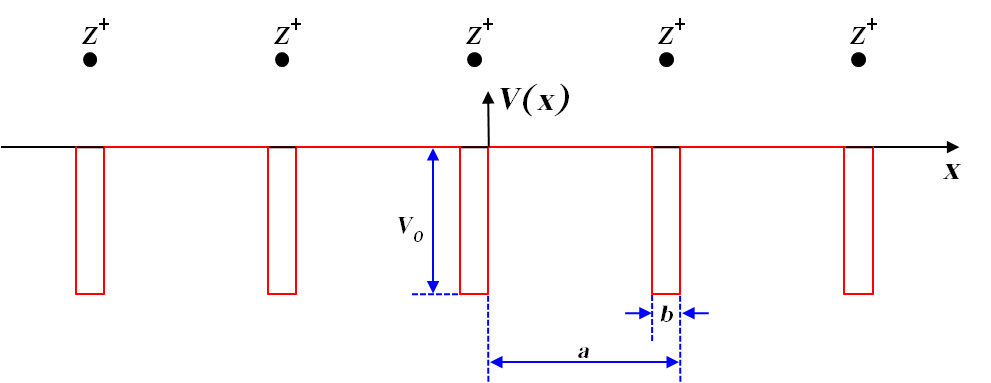
\includegraphics[width=0.75\textwidth]{Periodic_square_potential_130707} 
\end{figure*}
~\newpage % todo temporarily
The mathematical representation of the above is a multi-dimensional Schrödinger operator $A^{n}$ whose operation is formally defined by
\begin{equation}
	- \Delta + \rho \sum_{i \in \Z} \delta_{S_{i}} \label{the-operator-A-formally}
\end{equation}
on the whole of $\R^{n}$, where $\delta_{S_{i}}$ denotes the Dirac delta distribution on hypersurface $S_{i}$, that integrates any function $u \in L^{2}(\R)$ over the compact set $S_{i}$.
~\\ ~\\ 
Again motivated by the weak-formulation, given a right-hand side $f \in L^{2}(\R^{n})$ we consider for some $\mu \in \R$ the problem to find $u \in H^{1}(\R^{n})$ such that
	\begin{equation}
		\int_{\R^{n}} \nabla u \overline{\nabla v} + \rho \sum_{i \in \Z^{n}} \int_{S_{j}} u \overline{v} ds - \mu \int_{\R^{n}} u \overline{v} = \int_{Y} f \overline{v} \label{md-weak-formulation}
	\end{equation} 
holds for all $v \in H^{1}(\R^{n})$, where $s$ is the hypersurface measure associated to all $S_{j}$ \cite. 

\begin{remark}
	The term originating from the potential is finite as
	\[ \left| \sum_{j \in \Z^{n}} \int_{S_{j}} u \overline{v} \right|^{2} \leq \left( \sum_{j \in \Z^{n}} \| u \|_{L^{2}(S_{j})}^{2} \right) \left( \sum_{j \in \Z^{n}} \| v \|_{L^{2}(S_{j})}^{2} \right). \]
	Both terms on the right-hand side can be finitely estimated by the Trace theorem \cite[Chap. 5]{Evans98} as
	\[ \| u \|_{L^{2}(S_{j})}^{2} \leq 2 \left( \frac{1}{h} \|u\|_{L^{2}(B_{j})}^{2} + h \| \nabla u \|_{L^{2}(B_{j})}^{2} \right) \]
	for some $h > 0$. % todo more explicite
\end{remark}

We can once again exert Lax-Migram's Theorem to prove in \eqref{md-weak-formulation} the existence of a unique solution $u \in H^{1}(\R^{n})$ in \eqref{md-weak-formulation} for any $f \in L^{2}(\R^{n})$ if $\mu$ is small enough, define the operator injective $R_{\mu}^{n} \colon f \mapsto u$ and define $A$ by means of $R_{\mu}^{n}$.

\begin{remark}
	The operator $A$ is self-adjoint.	
\end{remark}


\begin{theorem}[Characterisation of $\mathcal{D}(A)$] Let $\Omega \coloneqq \R^{n} \setminus \overline{\bigcup_{j \in \Z^{n}} B_{j}}$. By choosing similar to above different functions $v \in C^{\infty}(\R^{n})$ in \eqref{md-weak-formulation} we can further characterise such $u \in \mathcal{D}(A)$, namely for all $j \in \Z^{n}$ it holds:
	\begin{enumerate}
		\item $\Delta u \in L^{2}(B_{j})$, $\Delta u \in L^{2}(\Omega)$ and $\sum_{j \in \Z^{n}} \|\Delta u \|_{L^{2}(B_{j})}^{2} < \infty$
		\item $u \big|_{S_{j} - 0} = u \big|_{S_{j} + 0}$
		\item $\frac{\partial u}{\partial \eta_{j}} \big|_{S_{j} - 0} - \frac{\partial u}{\partial \eta_{j}} \big|_{S_{j} + 0} - \rho u \big|_{S_{j}} = 0$ where $\eta_{j}$ denotes the normal on $S_{j}$
	\end{enumerate}
\end{theorem}

Now, restricting again this problem to a fundamental domain of periodicity, for example $Y$,
\begin{figure*}[h!] \centering
	  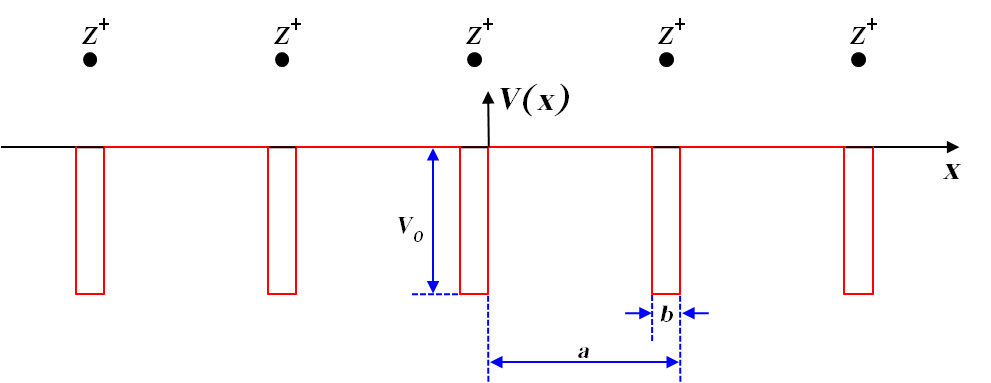
\includegraphics[width=0.75\textwidth]{Periodic_square_potential_130707} 
\end{figure*}

yields an operator $A^{n}_{k}$ which we can define by considering analogous to before the problem to find $u \in H^{1}_{k, n} \coloneqq \big\{ w \in H^{1}(Y) \colon w \big|_{S_{j}^{+}} = w \big|_{S_{j}^{+}} e^{i k_{j}}$ for $k \in [-\pi, \pi]^{2}, j = 1,2 \big\}$ such that
	\begin{equation}
		\int_{Y} \nabla u \overline{\nabla v} + \rho \int_{S} u \overline{v} ds - \mu \int_{Y} u \overline{v} = \int_{Y} f \overline{v}. \label{md-weak-formulation-res}
	\end{equation} 
for for all $v \in H^{1}_{k, n}$.
~\newline ~\newline
Again, Lax-Milgram's Theorem ensures the existence of a unique solution $u \in H^{1}_{k, n}$ if $\mu$ is small enough, and the operator $R_{\mu, k} \colon f \mapsto u$ is well-defined and injective. In return, this allows us to define 
	\[ A_{k}^{n} \coloneqq R_{\mu, k}^{n} + \mu I \]
The semi-periodic boundary conditions on $H^{1}_{k,n}$ require a solution $u \in H^{1}_{k, n}$ to \eqref{md-weak-formulation-res} to satisfy even
	\[ \frac{\partial u}{\partial x_{j}}\big|_{S_{j}^{+}} = e^{ik_{j}} \frac{\partial u}{\partial x_{j}}\big|_{S_{j}^{-}} \quad j = 1,2  \]
	
\begin{theorem}
	The operator $R_{\mu, k}^{n}$ on the fundamental domain of periodicity is compact.	

	\begin{proof}
		As in chapter \ref{chap3} used, the compact embedding yields the desired result, for a multi-dimensional proof see \cite[Chap. 4]{Adams}.	
	\end{proof}
\end{theorem}

By similar transformations of the problem \eqref{md-weak-formulation-res} as in \eqref{mod-eigv-problem} and \eqref{periodic-condition} we are able to show that the eigenvalues of $A^{n}_{k}$ are continuous functions of $k \in \overline{B}$, and thus $I_{s} = \{ \lambda_{s}(k) : k \in \overline{B} \}$ is a compact real interval for each $s \in \N$.
~\newline ~\newline
Ultimately, using the same arguments as in Chapter 4 based on Bloch waves, Floquet transform and a similar cut-off function $\eta$ as in \eqref{eta}, we are then able to prove the main result even for this multi-dimensional case, namely that the spectrum of a self-adjoint Schrödinger operator with periodic delta-potential on a hypersurface is the union of compact intervals, i.e.
	\[ \sigma(A) = \bigcup_{s \in \N} I_{s}. \]

\section{Outlook}	
	
We have to notice that we haven't determined the nature of the spectrum that is if there are possible gaps in the spectrum. However,... % todo schluss

\appendix
%\chapter*{Appendix} \cftaddtitleline{toc}{chapter}{Appendix}{}
\addcontentsline{toc}{section}{A.1 ~ Theorems}


\begin{atheorem}[Alternative definition of the Delta-Distribution] \label{athem:delta}
	For the sequence of functionals $\delta_{\epsilon}$ for $\epsilon > 0$, $x_{0} \in \R$ and $f \in \mathfrak{D}(\R)$ defined through $\delta_{\epsilon}(f) \coloneqq \frac{1}{\sqrt{2 \pi} \epsilon} \int_{\R} f(x) e^{-\frac{(x - x_{0})^{2}}{2 \epsilon^{2}}} dx$ it holds that  
 		\[ \delta_{x_{0}}(f) = \lim_{\epsilon \rightarrow 0} \delta_{\epsilon}(f). \]
	
	\begin{proof}
		By definition we have
			\[ \delta_{\epsilon}(f) = \frac{1}{\sqrt{2 \pi} \epsilon} \int_{-\infty}^{\infty} f(x) e^{-\frac{(x-x_{0})^{2}}{2 \epsilon^{2}}}dx. \]
		Substituting $z \coloneqq \frac{x - x_{0}}{\sqrt{2} \epsilon}$ yields
			\[ \frac{1}{\sqrt{2 \pi} \epsilon} \int_{-\infty}^{\infty} f(x) e^{-\frac{(x-x_{0})^{2}}{2 \epsilon^{2}}} dx = \frac{1}{\sqrt{2 \pi} \epsilon} \int_{-\infty}^{\infty} f(\sqrt{2} \epsilon z + x_{0}) e^{-z^{2}} dz. \]
		Now, using the Taylor series of $f$ around $x_{0}$ and a formula for the Gaussian integral we then get
			\[ \lim_{\epsilon \rightarrow 0} \frac{1}{\sqrt{\pi}} \int_{-\infty}^{\infty} e^{-z^{2}} \left( f(x_{0}) + \mathcal{O}(\epsilon) \right) dz = f(x_{0}) \frac{1}{\sqrt{\pi}} \int_{-\infty}^{\infty} e^{-z^{2}} dz = f(x_{0}). \]
	\end{proof}
\end{atheorem}

\begin{atheorem}[$L^{p}$-Approximation by test functions] \label{athm:approx}
	For $U \subseteq \R^{n}$ open, $C_{0}^{\infty}(U)$ is dense in $L^{p}(U)$, if $1 \leq p < \infty$.
	
	\begin{proof}
		See \cite[p. 31]{adams2003sobolev}.
	\end{proof}
\end{atheorem}

\begin{atheorem}[$H^{k}$-Approximation by test functions] \label{athm:hkapprox}
	Let $\Omega \subseteq \R^{n}$ be an open set. Let $u \in H^{k}(\Omega)$, then there exists a sequence of functions $u_{k} \in C^{\infty}(\Omega)$ such that $\| u_{k} - u \|_{H^{k}(\Omega)}$ as $n \rightarrow \infty$.
	% todo todo
	\begin{proof}
		See \cite[p. 138]{adams2003sobolev}.
	\end{proof}	
\end{atheorem}


\begin{atheorem}[Bessel's inequality] \label{athm:bessel}
	Let $H$ be a Hilbert space, and suppose that $e_1, e_2, ...$ is an orthonormal sequence in $H$. Then, for any $x \in H$ one has
	\[ \sum_{k=1}^{\infty}\left\vert\left\langle x,e_k\right\rangle_{H} \right\vert^2 \le \left\Vert x\right\Vert^2 \]
	where $\langle \cdot,\cdot \rangle_{H}$ denotes the inner product in the Hilbert space $H$.

	\begin{proof}
		See \cite[p. 233]{werner2006funkana}.
	\end{proof}
\end{atheorem}

\begin{atheorem}[Cauchy–Schwarz inequality] \label{athm:csi}
	For all vectors $u$ and $v$ of an inner product space it is true that
		\[ \left| \langle u,v \rangle \right|^{2} \leq \langle u,u \rangle \cdot \langle v,v \rangle, \]
	where $\langle \cdot ,\cdot \rangle$ is the inner product. 

	\begin{proof}
		See \cite[p. 20]{werner2006funkana}.
	\end{proof}
\end{atheorem}

\begin{atheorem}[Closed graph theorem] \label{athm:cgt}
	Let $X$ be a Banach space. Is $A$ a closed operator and $\mathcal{D}(A) = X$, then $A$ is continuous on $X$.

	\begin{proof}
		See \cite[p. 638]{evans1998partial}.
	\end{proof}
\end{atheorem}

\begin{atheorem}[Closeness of $H^{1}_{k}$ in $H^{1}(\Omega)$] \label{h1kclosed}
	$H^{1}_{k}$ is a closed subset1 of $H^{1}(\Omega)$, and therefore a Hilbert space with respect to the norm of $H^{1}(\Omega)$.
	
	\begin{proof} 
		Let $(f_{n})_{n \in \N}$ be a sequence in $H^{1}_{k}$ converging to $f \in H^{1}(\Omega)$. We already know that convergence with respect to the $H^{1}$-Norm implies convergence of the function and its derivative almost everywhere. Let us therefore define $g \coloneqq f - f_{n}$ then
		\begin{align*}
			\left| g \left(- \frac{1}{2} \right) \right|^{2} & \leq 2 |g(x)|^{2} + 2 \left( \int_{-\frac{1}{2}}^{x} |g'(\tau)| d\tau \right)^{2} \\
			& \leq 2 |g(x)|^{2} + 2 \int_{-\frac{1}{2}}^{\frac{1}{2}} |g'(\tau)|^{2} d\tau \\
			& \leq 2 \int_{-\frac{1}{2}}^{\frac{1}{2}} |g(\tau)|^{2} d\tau + 2 \int_{-\frac{1}{2}}^{\frac{1}{2}} |g'(\tau)|^{2} d\tau \\
			& = 2 \| g \|_{H^{1}(-\frac{1}{2}, \frac{1}{2})}^{2} \longrightarrow 0
		\end{align*}
		for $j \rightarrow \infty$, and analogously on the other boundary.
	\end{proof}
\end{atheorem}

\begin{atheorem}[Compact Embedding Theorem for Sobolev spaces] \label{compact-embedding-theorem} ~\
	\begin{enumerate}[label=\alph*\upshape)]
		\item Let $U \subseteq \R^{n}$ be a bounded open set of class $C^{1}$. Then the following compact embeddings hold:
			\begin{itemize}
				\item $H	^{1}(U) \subseteq L^{q}(U)$ for every $q \in [1, p^{*})$, where $n \geq 3$ and $p^{*} = \frac{2n}{n - 2}$.
				\item $H^{1}(U) \subseteq L^{q}(U)$ for every $q \in [1, \infty)$, if $n = 2$.
			\end{itemize}
		
			\begin{proof}
				Follows from Rellich-Kondrachov Compact Embedding Theorem, see \cite[p. 163]{precup2013linear} and \cite[p. 272]{evans1998partial}.
			\end{proof}
		\item Let $U \subseteq \R$ be a bounded, connected and open set. Then the embedding $H^{1}(U) \subseteq L^{2}(U)$ is compact.
			\begin{proof} 
				By Theorem \ref{embhc} $H^{1}(U) \subseteq C^{\frac{1}{2}}(U)$, hence we can estimate
					\begin{equation}
						|f(x) - f(y)| \leq c |x - y|^{\frac{1}{2}} \tag{$*$} \label{hoelderstet}
					\end{equation} 
				for some $c > 0$ and for all $x, y \in U$. Let $B_{H^{1}_{k}} \coloneqq \{ f \in H^{1}_{k}(U) : \|f\|_{H^{1}(U)} \leq 1 \}$, then for $f \in B_{H^{1}_{k}}$ it holds that
				\begin{equation}
					|f(x)|^{2} \leq 2 \| f\|^{2}_{L^{2}(U)} + 2 \leq 4 \quad \forall x \in U. \tag{$**$} \label{eqbounded}
				\end{equation} 
				For an arbitrary $\epsilon > 0$ we now partition $U$ into $n_{\epsilon}$ equidistant, disjoint intervals $I_{k}$, i.e. $U = \bigcup_{k = 1}^{n_{\epsilon}} I_{k}$. Since all $f \in B_{H^{1}_{k}}$ are uniformly bounded on $U$ by \eqref{eqbounded}, there exist for each subinterval $I_{k}$ a finite number of constants $c_{1, k}, \dotsc, c_{\nu_{\epsilon}, k}$ such that
					\[ \forall f \in B_{H^{1}_{k}} ~\exists j \in \{1, \dotsc, \nu_{\epsilon} \} : \left| f\left(\frac{k}{n_{\epsilon}}\right) - c_{j, k} \right| < \frac{1}{n_{\epsilon}} ~\forall k \in \{ 1, \dotsc, n_{\epsilon} \}. \]
				Therefore, there are finitely many step functions such that for any $f \in L^{2}(U)$ there exists one of those step functions $g \in L^{2}(U)$, with function value $c_{k}$ on subinterval $I_{k}$ for each $k \in \{1, \dotsc, n_{\epsilon}\}$, such that by \eqref{hoelderstet}
				\begin{align*}
					\| f - g\|^{2}_{L^{2}(U)} & = \sum_{k=0}^{n_{\epsilon}-1} \int_{\frac{k}{n_{\epsilon}}}^{\frac{k+1}{n_{\epsilon}}} |f(x) - c_{k+1}|^{2} dx \\
					& \leq 2 \sum_{k=0}^{n_{\epsilon}-1} \int_{\frac{k}{n_{\epsilon}}}^{\frac{k+1}{n_{\epsilon}}} \left|f(x) - f\left(\frac{k}{n_{\epsilon}}\right)\right|^{2} dx + 2 \sum_{k=0}^{n_{\epsilon}-1} \int_{\frac{k}{n_{\epsilon}}}^{\frac{k+1}{n_{\epsilon}}} \left| f\left(\frac{k}{n_{\epsilon}}\right) - c_{k+1} \right|^{2} dx \\ 
					& \leq 2 \sum_{k = 0}^{n_{\epsilon}-1} \frac{c}{n_{\epsilon}^{2}} + 2 \sum_{k = 0}^{n_{\epsilon}-1} \frac{1}{n_{\epsilon}^{3}} = \frac{2}{n_{\epsilon}} \left( c + \frac{1}{n_{\epsilon}} \right) < \epsilon
				\end{align*}
				for $n_{\epsilon}$ large enough. This means, in conclusion, that $B_{H^{1}_{k}}$ is totally bounded in $L^{2}(U)$ and in return, since $H^{1}_{k}$ is closed, it can be compactly embedded in $L^{2}(U)$.
			\end{proof}
	\end{enumerate}
\end{atheorem}

\begin{atheorem}[Dominated Convergence Theorem] \label{athm:domconvthm}
	Let ${f_n}$ be a sequence of real-valued measurable functions on a measure space $(S, \Sigma, \mu)$. Suppose that the sequence converges pointwise to a function $f$ and is dominated by some integrable function $g$ in the sense that
		\[ |f_n(x)| \le g(x) \]
	for all numbers n in the index set of the sequence and all points $x \in S$. Then f is integrable and
		\[ \lim_{n\to\infty} \int_S |f_n-f|\,d\mu = 0 \]
	which also implies $\lim_{n\to\infty} \int_S f_n\,d\mu = \int_S f\,d\mu$.

	\begin{proof}
		See \cite[p. 516]{werner2006funkana}.
	\end{proof}
\end{atheorem}

\begin{atheorem}[Eigenvectors of a compact, symmetric operator] \label{eigvcso}
	Let $H$ be a separable Hilbert space, and suppose $S \colon H \rightarrow H$ is a compact and symmetric operator. Then there exists a countable orthonormal basis of $H$ consisting of eigenvectors of $S$.
	
	\begin{proof}
		See \cite[p. 645]{evans1998partial}.
	\end{proof}
\end{atheorem}

\begin{atheorem}[Embedding of $H^{1}$ in $C^{\frac{1}{2}}$] \label{embhc}
	Let $[a, b]$ be a compact interval in $\R$. Then, $H^{1}([a, b])$ is embedded in $C^{\frac{1}{2}}([a, b])$
	
	\begin{proof}
		See \cite[p. 269]{evans1998partial}.
	\end{proof}
\end{atheorem}

\begin{atheorem}[Equivalent definitions of closed operators] % todo  kein Label
	Let X, Y be two Banach spaces. A linear operator $A \colon X \supset \mathcal{D}(A)  \rightarrow Y$ is closed if for every sequence $(x_n)_{n \in \N}$ in $\mathcal{D}(A)$ from
	\[ x_{n} \rightarrow x \in X \text{ and } Tx_{n} \rightarrow y \in Y \]
	follows that $x \in D$ and $Tx = y$.

	\begin{proof}
		 See \cite[p. 156]{werner2006funkana}.
	\end{proof}
\end{atheorem}	

\begin{atheorem}[Fubini's Theorem for integrable functions] \label{athm:fubini}
	Suppose $X$ and $Y$ are $\sigma$-finite measure spaces, and suppose that $X \times Y$ is given the product measure (which is unique as $X$ and $Y$ are $\sigma$-finite). Fubini's Theorem states that if $f(x,y)$ is $X \times Y$ integrable, meaning that it is measurable and
		\[  \int_{X\times Y} |f(x,y)|\,\text{d}(x,y)<\infty, \]
	then
		\[ \int_X\left(\int_Y f(x,y)\,\text{d}y\right)\,\text{d}x=\int_Y\left(\int_X f(x,y)\,\text{d}x\right)\,\text{d}y=\int_{X\times Y} f(x,y)\,\text{d}(x,y). \]
	The first two integrals are iterated integrals with respect to two measures, respectively, and the third is an integral with respect to the product measure

	\begin{proof}
		See \cite[p. 514]{werner2006funkana}.
	\end{proof}
\end{atheorem}

\begin{atheorem}[Lax-Milgram] \label{athm:lm}
	Let $H$ be a Hilbert space where $\| \cdot \|$ denotes the norm on $H$, and let $B \colon H \times H \rightarrow \C$ be a sesquilinear form. If there exist constants $\alpha, \beta > 0$ such that
	\begin{enumerate}[label=\alph*\upshape)]
		\item $\left| B[u, v] \right| \leq \alpha \| u \| \|v \| \quad (u, v \in H)$ and
		\item $Re(B[u,u]) \geq \beta \|u\|^{2} \quad (u \in H)$,
	\end{enumerate}
	then there exists to each $l \in H^{*}$ a unique $w \in H$ such that
		\[ B[v, w] = l(v) \]
	hold for all $v \in H$.
		
	\begin{proof}
		See \cite[Amd to problem 51]{plum2015dglhr}.
	\end{proof}
\end{atheorem}

\begin{atheorem}[Monotone Convergence Theorem] \label{athm:monotonconvthm}
	Let $(X, \Sigma, \mu)$ be a measure space. Let $f_1, f_2, \ldots$  be a pointwise non-decreasing sequence of $[0, \infty]$-valued $\Sigma$–measurable functions, i.e. for every $k \geq 1$ and every $x$ in $X$,
		\[ 0 \leq f_k(x) \leq f_{k+1}(x). \] 
	Next, set the pointwise limit of the sequence $(f_{n})$ to be $f$. That is, for every $x$ in $X$,
		\[ f(x):= \lim_{k\to\infty} f_k(x). \]
	Then $f$ is $\Sigma$–measurable and
		\[ \lim_{k\to\infty} \int f_k \, \mathrm{d}\mu = \int f \, \mathrm{d}\mu. \]

	\begin{proof}
		See \cite[p. 516]{werner2006funkana}.
	\end{proof}
\end{atheorem}

\begin{atheorem}[Orthonormality of $\vartheta$] \label{athm:eta}
	The sequence
		\[ \vartheta_{n}(k) \coloneqq \frac{1}{\sqrt{|B|}} e^{ikn} \]
	forms an orthonormal basis of $L^{2}(B)$.

	\begin{proof}
		 For $m, n \in \N$ we see that
		 \[ \langle \vartheta_{n}, \vartheta_{m} \rangle_{L^{2}(B)} = \frac{1}{|B|} \int_{B} e^{ikn} \overline{e^{ikm}} dk = \frac{1}{|B|} \int_{B} e^{ik(n-m)} dk = \begin{cases} 0 & \text{ for } n \neq m \\ 1 & \text{ for } n = m, \end{cases} \]
		 hence the asserted follows.
	\end{proof}
\end{atheorem}

\begin{atheorem}[Parseval's identity] \label{athm:parseval}
	Suppose that $H$ is a Hilbert space with inner product $\langle \cdot,\cdot \rangle$. Let $(e_{n})$ be an orthonormal basis of $H$; i.e., the linear span of the $e_n$ is dense in $H$, and the $e_n$ are mutually orthonormal:
		\[ \langle e_{m},e_{n}\rangle ={\begin{cases}1&{\mbox{if}}\ m=n\\0&{\mbox{if}}\ m\not =n.\end{cases}} \]
	Then Parseval's identity asserts that for every $x \in H$,
		\[ \sum _{n}|\langle x,e_{n}\rangle |^{2}=\|x\|^{2}.\]

	\begin{proof}
		See \cite[p. 236]{werner2006funkana}.
	\end{proof}
\end{atheorem}

\begin{atheorem}[Poincare's inequality] \label{poincareineq}
 If a domain $\Omega \subset \R^{n}$ has finite width, then there exists a constant $c = c(p)$ such that for all $\varphi \in C_{0}^{\infty}(\Omega)$
 	\[ \| \varphi \|_{L^{p}(\Omega)} \leq c \| \nabla \varphi \|_{L^{p}(\Omega)} \]
 	With Theorem \ref{athm:approx} this can be extended to every function $u \in L^{p}(\Omega)$.
 	
	\begin{proof}
		See \cite[p. 183]{adams2003sobolev}.
	\end{proof}
\end{atheorem}

\begin{atheorem}[Poincare's min-max principle for eigenvalues] \label{athm:poincare}
	Let $X$ be a seperable Hilbert space and $\langle \cdot, \cdot \rangle_{X}$ denote the scalar product on $X$. Let $A \colon \mathcal{D}(A) \rightarrow X$ be a self-adjoint operator where $\mathcal{D}(A) \subseteq X$. If the set of eigenvalues $\lambda_{s}$ is at most countable, then
	\begin{equation*}
			\lambda_{s} = \underset{\dim U = s}{\min_{U \subseteq \mathcal{D}(A)}} \max_{v \in U \setminus \{ 0 \} } \frac{\langle A v, v \rangle_{X}}{\langle v, v \rangle_{X}}. 
	\end{equation*} 

	\begin{proof}
		See \cite[p. 119]{teschl2014mathematical}.
	\end{proof}
\end{atheorem}

\begin{atheorem}[Properties of self-adjoint operators] ~\ \label{athm:propself}
	\begin{enumerate}[label=\alph*\upshape)]
		\item Every self-adjoint is symmetric and closed.
			\begin{proof}
				 Follows directly from the definitions for self-adjoint and closed operators.
			\end{proof}
		\item For $A$ being a self-adjoint operator, $\lambda \in \rho(A)$, $(A - \lambda I)^{-1}$ is bounded.
			\begin{proof}
				Since every self-adjoint is closed, $(A - \lambda I)$ is as the shift with $\lambda \in \R$ also closed. Furthermore, the graph of $(A - \lambda I)^{-1}$ is simply the graph of $(A - \lambda I)$ rotated and hence $(A - \lambda I)^{-1}$ is closed as well. The closed Graph Theorem now yields the desired result.
			\end{proof}
	\end{enumerate}
\end{atheorem}

\begin{atheorem}[Properties of the resolvent set]
	The resolvent set $\rho(A) \subseteq \mathbb{C}$ of a bounded linear operator $A$ is an open set.
	
	\begin{proof}
		See \cite[p. 259]{werner2006funkana}.
	\end{proof}
\end{atheorem}

\begin{atheorem}[The spectrum of self-adjoint operators] \label{spectrul-sa-real}
	The spectrum of a self-adjoint operator $A$ is real. 
	
	\begin{proof}
		Let $\lambda$ be an eigenvalue of $A$, i.e. there exists $x \in X$ such that $A x = \lambda x$. From this it follows that $\langle A x, x \rangle = \langle \lambda x , x \rangle$. Using then the fact that $A$ is self-adjoint we can further deduce
		\[ \lambda \langle x , x \rangle = \langle \lambda x , x \rangle = \langle A x, x \rangle = \langle x, A x \rangle = \langle x , \lambda x \rangle = \overline{\lambda} \langle  x , x \rangle \]
		Hence, $\lambda = \overline{\lambda}$, which shows the desired result.
	\end{proof}
\end{atheorem}

\begin{atheorem}[Trace Theorem] \label{athm:trace}
	Assume $U$ is bounded and $\partial U$ is $C^{1}$. Then there exists a bounded linear operator
		\[ T \colon H^{1}(U) \rightarrow L^{2}(\partial U) \]
	such that
	\begin{enumerate}[label=\alph*\upshape)]
		\item $Tu = u\big|_{\partial U}$ if $u \in H^{1}(U) \cap C(\overline{U})$
		\item $\|Tu\|_{L^{2}(\partial U)} \leq C \|u\|_{H^{1}(U)}$
	\end{enumerate}
	for each $u \in H^{1}(U)$, with the constant $C$ depending only on $U$.
	
	\begin{proof}
		See \cite[p. 258]{evans1998partial}.
	\end{proof}
\end{atheorem}

\begin{atheorem}[Uniqueness of weak derivatives] \label{athem:uniqueness_of_weak_deriv}
	Let $\Omega \subseteq \R$ be open, if it exists, the $\alpha$-th weak derivative of $u$ is uniquely determined up to a set of measure zero.
	
	\begin{proof}
		Assume that $g, \tilde{g} \in L_{loc}^{1}(\Omega)$ satisfy for all $\varphi \in C_{0}^{\infty}(\Omega)$
		\[ (-1)^{\alpha} \int_{\Omega} f \varphi' = \int_{\Omega} g \varphi  = \int_{\Omega} \tilde{g} \varphi. \]
		Then $\int_{\Omega} \left( g - \tilde{g} \right) \varphi = 0$ for all $\varphi \in C_{0}^{\infty}(\Omega)$, whence $g - \tilde{g} = 0$ almost everywhere.	
	\end{proof}
\end{atheorem} 
\begin{thebibliography}{00}
  \bibitem{Plum10} A. Lechleiter, M. Plum, G. Schneider and C. Wieners, {\it Photonic Crystals: Mathematical Analysis and Numerical Approximation}. Birkh{\"a}user 2010.
  \bibitem{Kuchment} P. Kuchment, {\it An Overview of Periodic Elliptic Operators} Bulletin of the American Mathematical Society 2016.
  \bibitem{Evans98} L. C. Evans, {\it Photonic Partial Differential Equations}. Oxford University Press 1998, Volume 19.
  \bibitem{WernerFA} D. Werner, {\it Funktionalanalysis}. Springer 2011, Volume 7.
  \bibitem{Adams} R. Adams, {\it Sobolev spaces}. Academic Press New York 1975.
  \bibitem{AlbSMQM} S. Albeverio, F. Gesztesy, R. Hoegh-Krohn, H. Holden, {\it Solvable Models in Quantum Mechanics}. AMS Chelsea Publishing Second edition, 2005.
  \bibitem{Federer} H. Federer, {\it Colloquium Lectures on Geometric Measure} Bulletin of the American Mathematical Society 1978.
  \bibitem{HeeringEP} W. Heering, {\it Elektrophysik}. Lecture, Karlsruhe Institute of Technology, 2002.
  \bibitem{PlumVL} M. Plum {\it Differentialgleichungen und Hilberträume}. Lecture, Karlsruhe Institute of Technology, 2015.
  \bibitem{WeisFA} L. Weis, {\it Funktionalanalysis}. Lecture, Karlsruhe Institute of Technology, 2015.
  \bibitem{WeisST} L. Weis, {\it Spektraltheorie}. Lecture, Karlsruhe Institute of Technology, 2016.
\end{thebibliography} 
\thispagestyle{empty}


\vspace*{8cm}


\section*{Erklärung}

Hiermit versichere ich, dass ich diese Arbeit selbständig verfasst und keine anderen, als die angegebenen Quellen und Hilfsmittel benutzt, die wörtlich oder inhaltlich übernommenen Stellen als solche kenntlich gemacht und die Satzung des Karlsruher Instituts für Technologie zur Sicherung guter wissenschaftlicher Praxis in der jeweils gültigen Fassung beachtet habe. \\[2ex] 

\noindent
Ort, den Datum\\[5ex]

% Unterschrift (handgeschrieben)


\end{document}